\documentclass[11pt]{article}
\usepackage[utf8]{inputenc}
\usepackage[T1]{fontenc}
\usepackage{textcomp}
\usepackage[a4paper,margin=2.1cm]{geometry}
\usepackage{amsmath,amssymb}
\usepackage{cancel}
\usepackage{graphicx}
\usepackage{tikz}
\usetikzlibrary{positioning,arrows.meta}
\usepackage{xcolor}
\usepackage{mdframed}
\usepackage[colorlinks=true,linkcolor=blue!60!black]{hyperref}
\setlength{\parindent}{0pt}
\setlength{\parskip}{6pt}

\newcommand{\question}[1]{\par\medskip\noindent\textbf{#1}\par}
\newmdenv[linecolor=green!45!black,linewidth=0.8pt,backgroundcolor=green!4,
  innertopmargin=4pt,innerbottommargin=4pt,skipabove=6pt,skipbelow=6pt]{answerbox}

\title{\textbf{Algebraic Fractions}\\[0.3em]\large Worked Solutions with TikZ Diagrams}
\author{Wisest Maths --- Year 1 A-Level, Algebra (ref \texttt{a3})}
\date{}

\begin{document}
\maketitle
\noindent This document contains all 52 \emph{Algebraic Fractions} questions, each with a fully
worked solution and a TikZ diagram chosen to match the operation:
\begin{itemize}\setlength{\itemsep}{1pt}
  \item \textbf{Cancellation} diagrams (factorise, then strike the common factor) for \emph{simplifying} a single fraction;
  \item \textbf{Cross-multiplication} (butterfly) diagrams for \emph{adding or subtracting} two fractions;
  \item \textbf{Solution-flow} diagrams (one operation per arrow) for \emph{multiplying/dividing} and for common-denominator work with three or more terms.
\end{itemize}
\tableofcontents
\bigskip
\hrule

\section*{Algebraic Fractions 1\quad\small\texttt{(a3-001)}}
\addcontentsline{toc}{section}{Algebraic Fractions 1 (a3-001)}
\textit{Difficulty: Foundation \quad\textbar\quad Marks: 2}

\question{Simplify the expression: \( \frac{2x+10}{6} \)}

\textbf{Worked solution.}

\textit{Step 1: Factorise the numerator by extracting the highest common factor of 2.}
\[\begin{gathered}
\frac{2(x + 5)}{6}
\end{gathered}\]
Identify the common factor in the top expression to prepare for cancellation.

\textit{Step 2: Cancel the common factor of 2 from both the numerator and the denominator.}
\[\begin{gathered}
\frac{x + 5}{3}
\end{gathered}\]
Divide the top and bottom by 2.

\begin{answerbox}
\textbf{Final answer:}\quad \(\displaystyle \frac{x + 5}{3}\)
\end{answerbox}
\textbf{Diagram.}

\begin{center}
\resizebox{\ifdim\width>\linewidth \linewidth\else \width\fi}{!}{%
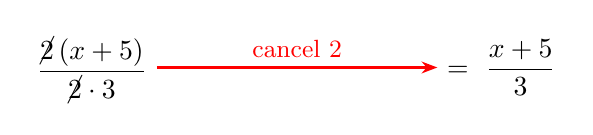
\begin{tikzpicture}[>={Stealth[length=2mm]}]
\node (f) {$\displaystyle \frac{\cancel{2}\,(x+5)}{\cancel{2}\cdot 3}$};
\node (r) at (5.2,0) {$\displaystyle =\ \frac{x+5}{3}$};
\draw[->,red,thick] (f.east) -- (r.west) node[midway,above,font=\small]{cancel $2$};
\end{tikzpicture}
}
\end{center}
\small Cancellation diagram: factorise top and bottom, then strike the common factor.\normalsize

\medskip\hrule

\section*{Algebraic Fractions 2\quad\small\texttt{(a3-002)}}
\addcontentsline{toc}{section}{Algebraic Fractions 2 (a3-002)}
\textit{Difficulty: Foundation \quad\textbar\quad Marks: 2}

\question{Simplify fully: \( \frac{np^2 - 2n^2p}{np} \)}

\textbf{Worked solution.}

\textit{Step 1: Factorise the numerator completely by taking out the common factor of \( np \).}
\[\begin{gathered}
\frac{np(p - 2n)}{np}
\end{gathered}\]
Find the highest common algebraic factors in the top expression.

\textit{Step 2: Cancel the \( np \) term from both the numerator and the denominator.}
\[\begin{gathered}
p - 2n
\end{gathered}\]
Divide the expression by the common term.

\begin{answerbox}
\textbf{Final answer:}\quad \(\displaystyle p - 2n\)
\end{answerbox}
\textbf{Diagram.}

\begin{center}
\resizebox{\ifdim\width>\linewidth \linewidth\else \width\fi}{!}{%
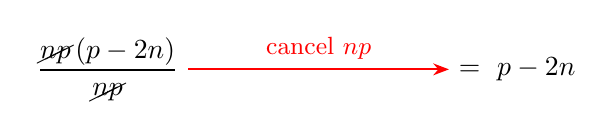
\begin{tikzpicture}[>={Stealth[length=2mm]}]
\node (f) {$\displaystyle \frac{\cancel{np}\,(p-2n)}{\cancel{np}}$};
\node (r) at (5.2,0) {$\displaystyle =\ p-2n$};
\draw[->,red,thick] (f.east) -- (r.west) node[midway,above,font=\small]{cancel $np$};
\end{tikzpicture}
}
\end{center}
\small Cancellation diagram: factorise top and bottom, then strike the common factor.\normalsize

\medskip\hrule

\section*{Algebraic Fractions 3\quad\small\texttt{(a3-003)}}
\addcontentsline{toc}{section}{Algebraic Fractions 3 (a3-003)}
\textit{Difficulty: Foundation \quad\textbar\quad Marks: 2}

\question{Express as a single fraction: \( \frac{x}{3} + \frac{x}{4} \)}

\textbf{Worked solution.}

\textit{Step 1: Find a common denominator for the fractions, which is 12. Multiply the top and bottom of the first fraction by 4, and the second by 3.}
\[\begin{gathered}
\frac{4x}{12} + \frac{3x}{12}
\end{gathered}\]
Rewrite the fractions so they can be combined.

\textit{Step 2: Add the numerators together over the common denominator.}
\[\begin{gathered}
\frac{7x}{12}
\end{gathered}\]
Combine the like terms on the top line.

\begin{answerbox}
\textbf{Final answer:}\quad \(\displaystyle \frac{7x}{12}\)
\end{answerbox}
\textbf{Diagram.}

\begin{center}
\resizebox{\ifdim\width>\linewidth \linewidth\else \width\fi}{!}{%
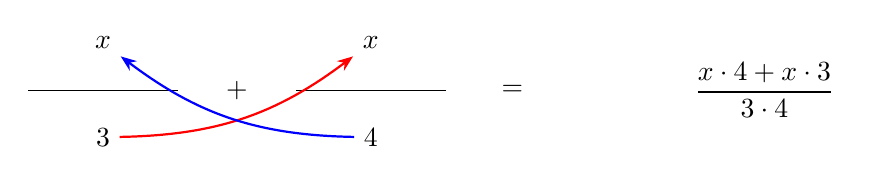
\begin{tikzpicture}[>={Stealth[length=2mm]}]
\node (a) at (0,0.6) {$x$};
\draw (-0.95,0) -- (0.95,0);
\node (b) at (0,-0.6) {$3$};
\node at (1.7,0) {$+$};
\node (c) at (3.4,0.6) {$x$};
\draw (2.45,0) -- (4.35,0);
\node (d) at (3.4,-0.6) {$4$};
\node at (5.2,0) {$=$};
\node at (8.4,0) {$\displaystyle \frac{x\cdot 4 + x\cdot 3}{3\cdot 4}$};
\draw[->,red,thick] (b) to[bend right=18] (c);
\draw[->,blue,thick] (d) to[bend left=18] (a);
\end{tikzpicture}
}
\end{center}
\small Cross-multiplication: each numerator multiplies the \emph{other} denominator (curved arrows); the denominators multiply to give the common denominator.\normalsize

\medskip\hrule

\section*{Algebraic Fractions 4\quad\small\texttt{(a3-004)}}
\addcontentsline{toc}{section}{Algebraic Fractions 4 (a3-004)}
\textit{Difficulty: Foundation \quad\textbar\quad Marks: 2}

\question{Express as a single fraction: \( \frac{1}{2p} - \frac{1}{5q} \)}

\textbf{Worked solution.}

\textit{Step 1: Find a common denominator by multiplying the two denominators together to get \( 10pq \).}
\[\begin{gathered}
\frac{5q}{10pq} - \frac{2p}{10pq}
\end{gathered}\]
Multiply the top and bottom of each fraction by the missing factors.

\textit{Step 2: Subtract the numerators over the common denominator.}
\[\begin{gathered}
\frac{5q - 2p}{10pq}
\end{gathered}\]
Combine the terms on the top line into a single expression.

\begin{answerbox}
\textbf{Final answer:}\quad \(\displaystyle \frac{5q - 2p}{10pq}\)
\end{answerbox}
\textbf{Diagram.}

\begin{center}
\resizebox{\ifdim\width>\linewidth \linewidth\else \width\fi}{!}{%
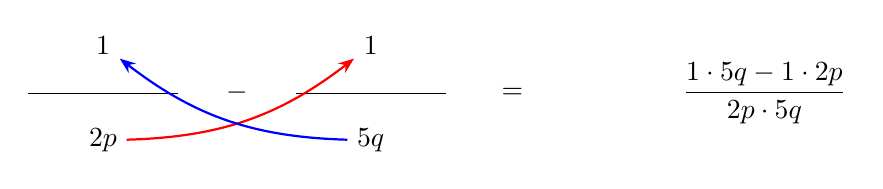
\begin{tikzpicture}[>={Stealth[length=2mm]}]
\node (a) at (0,0.6) {$1$};
\draw (-0.95,0) -- (0.95,0);
\node (b) at (0,-0.6) {$2p$};
\node at (1.7,0) {$-$};
\node (c) at (3.4,0.6) {$1$};
\draw (2.45,0) -- (4.35,0);
\node (d) at (3.4,-0.6) {$5q$};
\node at (5.2,0) {$=$};
\node at (8.4,0) {$\displaystyle \frac{1\cdot 5q - 1\cdot 2p}{2p\cdot 5q}$};
\draw[->,red,thick] (b) to[bend right=18] (c);
\draw[->,blue,thick] (d) to[bend left=18] (a);
\end{tikzpicture}
}
\end{center}
\small Cross-multiplication: each numerator multiplies the \emph{other} denominator (curved arrows); the denominators multiply to give the common denominator.\normalsize

\medskip\hrule

\section*{Algebraic Fractions 5\quad\small\texttt{(a3-005)}}
\addcontentsline{toc}{section}{Algebraic Fractions 5 (a3-005)}
\textit{Difficulty: Foundation \quad\textbar\quad Marks: 3}

\question{Express as a single fraction in its simplest form: \( \frac{5}{y-1} + \frac{3}{y-2} \)}

\textbf{Worked solution.}

\textit{Step 1: Find the common denominator by multiplying the two denominators together: \( (y-1)(y-2) \). Rewrite each fraction.}
\[\begin{gathered}
\frac{5(y-2)}{(y-1)(y-2)} + \frac{3(y-1)}{(y-1)(y-2)}
\end{gathered}\]
Multiply the top and bottom of each fraction by the opposite denominator.

\textit{Step 2: Combine the numerators over the common denominator and expand the brackets.}
\[\begin{gathered}
\frac{5y - 10 + 3y - 3}{(y-1)(y-2)}
\end{gathered}\]
Bring the fractions together and multiply out the terms on top.

\textit{Step 3: Simplify the numerator by collecting like terms: \( 5y + 3y = 8y \) and \( -10 - 3 = -13 \).}
\[\begin{gathered}
\frac{8y - 13}{(y-1)(y-2)}
\end{gathered}\]
Neaten the top line to get the final answer.

\begin{answerbox}
\textbf{Final answer:}\quad \(\displaystyle \frac{8y - 13}{(y-1)(y-2)}\)
\end{answerbox}
\textbf{Diagram.}

\begin{center}
\resizebox{\ifdim\width>\linewidth \linewidth\else \width\fi}{!}{%
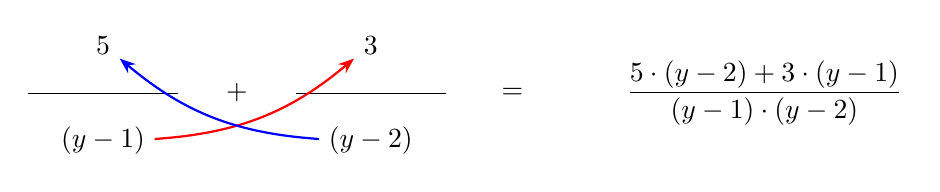
\begin{tikzpicture}[>={Stealth[length=2mm]}]
\node (a) at (0,0.6) {$5$};
\draw (-0.95,0) -- (0.95,0);
\node (b) at (0,-0.6) {$(y-1)$};
\node at (1.7,0) {$+$};
\node (c) at (3.4,0.6) {$3$};
\draw (2.45,0) -- (4.35,0);
\node (d) at (3.4,-0.6) {$(y-2)$};
\node at (5.2,0) {$=$};
\node at (8.4,0) {$\displaystyle \frac{5\cdot (y-2) + 3\cdot (y-1)}{(y-1)\cdot (y-2)}$};
\draw[->,red,thick] (b) to[bend right=18] (c);
\draw[->,blue,thick] (d) to[bend left=18] (a);
\end{tikzpicture}
}
\end{center}
\small Cross-multiplication: each numerator multiplies the \emph{other} denominator (curved arrows); the denominators multiply to give the common denominator.\normalsize

\medskip\hrule

\section*{Algebraic Fractions 6\quad\small\texttt{(a3-006)}}
\addcontentsline{toc}{section}{Algebraic Fractions 6 (a3-006)}
\textit{Difficulty: Foundation \quad\textbar\quad Marks: 3}

\question{Express as a single fraction in its simplest form: \( \frac{7}{r-5} - \frac{4}{r+3} \)}

\textbf{Worked solution.}

\textit{Step 1: Find the common denominator: \( (r-5)(r+3) \). Multiply the numerator of each fraction by the denominator of the other.}
\[\begin{gathered}
\frac{7(r+3)}{(r-5)(r+3)} - \frac{4(r-5)}{(r-5)(r+3)}
\end{gathered}\]
Create equivalent fractions with the same denominator.

\textit{Step 2: Combine the numerators and expand the brackets. Pay close attention to expanding the negative term: \( -4(r-5) = -4r + 20 \).}
\[\begin{gathered}
\frac{7r + 21 - 4r + 20}{(r-5)(r+3)}
\end{gathered}\]
Distribute the values across the brackets on the top line.

\textit{Step 3: Collect like terms on the numerator to fully simplify the expression.}
\[\begin{gathered}
\frac{3r + 41}{(r-5)(r+3)}
\end{gathered}\]
Combine the \( r \) terms and the number terms.

\begin{answerbox}
\textbf{Final answer:}\quad \(\displaystyle \frac{3r + 41}{(r-5)(r+3)}\)
\end{answerbox}
\textbf{Diagram.}

\begin{center}
\resizebox{\ifdim\width>\linewidth \linewidth\else \width\fi}{!}{%
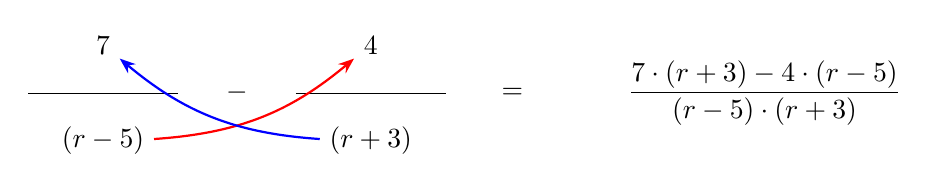
\begin{tikzpicture}[>={Stealth[length=2mm]}]
\node (a) at (0,0.6) {$7$};
\draw (-0.95,0) -- (0.95,0);
\node (b) at (0,-0.6) {$(r-5)$};
\node at (1.7,0) {$-$};
\node (c) at (3.4,0.6) {$4$};
\draw (2.45,0) -- (4.35,0);
\node (d) at (3.4,-0.6) {$(r+3)$};
\node at (5.2,0) {$=$};
\node at (8.4,0) {$\displaystyle \frac{7\cdot (r+3) - 4\cdot (r-5)}{(r-5)\cdot (r+3)}$};
\draw[->,red,thick] (b) to[bend right=18] (c);
\draw[->,blue,thick] (d) to[bend left=18] (a);
\end{tikzpicture}
}
\end{center}
\small Cross-multiplication: each numerator multiplies the \emph{other} denominator (curved arrows); the denominators multiply to give the common denominator.\normalsize

\medskip\hrule

\section*{Algebraic Fractions 7\quad\small\texttt{(a3-007)}}
\addcontentsline{toc}{section}{Algebraic Fractions 7 (a3-007)}
\textit{Difficulty: Foundation \quad\textbar\quad Marks: 4}

\question{Simplify the expression fully: \( \frac{4g^2 - 4h^2}{g^2 + gh} \)}

\textbf{Worked solution.}

\textit{Step 1: Factorise the numerator by extracting the common factor of 4.}
\[\begin{gathered}
\frac{4(g^2 - h^2)}{g^2 + gh}
\end{gathered}\]
Always look for the highest common numerical factor first.

\textit{Step 2: Notice the bracket on the top is a difference of two squares. Factorise it fully. Also factorise the denominator by extracting \( g \).}
\[\begin{gathered}
\frac{4(g-h)(g+h)}{g(g+h)}
\end{gathered}\]
Break down both the top and bottom expressions into their factored forms.

\textit{Step 3: Cancel the common binomial factor of \( (g+h) \) from the numerator and denominator.}
\[\begin{gathered}
\frac{4(g-h)}{g}
\end{gathered}\]
Divide the top and bottom by the shared bracket.

\begin{answerbox}
\textbf{Final answer:}\quad \(\displaystyle \frac{4(g-h)}{g}\)
\end{answerbox}
\textbf{Diagram.}

\begin{center}
\resizebox{\ifdim\width>\linewidth \linewidth\else \width\fi}{!}{%
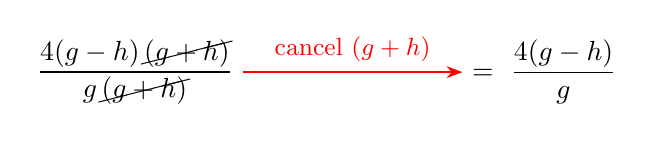
\begin{tikzpicture}[>={Stealth[length=2mm]}]
\node (f) {$\displaystyle \frac{4(g-h)\,\cancel{(g+h)}}{g\,\cancel{(g+h)}}$};
\node (r) at (5.2,0) {$\displaystyle =\ \frac{4(g-h)}{g}$};
\draw[->,red,thick] (f.east) -- (r.west) node[midway,above,font=\small]{cancel $(g+h)$};
\end{tikzpicture}
}
\end{center}
\small Cancellation diagram: factorise top and bottom, then strike the common factor.\normalsize

\medskip\hrule

\section*{Algebraic Fractions 8\quad\small\texttt{(a3-008)}}
\addcontentsline{toc}{section}{Algebraic Fractions 8 (a3-008)}
\textit{Difficulty: Foundation \quad\textbar\quad Marks: 2}

\question{Simplify the expression fully: \( \frac{15m - 10}{5} \)}

\textbf{Worked solution.}

\textit{Step 1: Factorise the numerator by extracting the highest common factor, which is 5.}
\[\begin{gathered}
\frac{5(3m - 2)}{5}
\end{gathered}\]
Look for the largest number that divides exactly into both 15m and 10.

\textit{Step 2: Cancel the common factor of 5 from the numerator and the denominator.}
\[\begin{gathered}
3m - 2
\end{gathered}\]
Dividing the top and bottom by 5 leaves the expression in the bracket.

\begin{answerbox}
\textbf{Final answer:}\quad \(\displaystyle 3m - 2\)
\end{answerbox}
\textbf{Diagram.}

\begin{center}
\resizebox{\ifdim\width>\linewidth \linewidth\else \width\fi}{!}{%
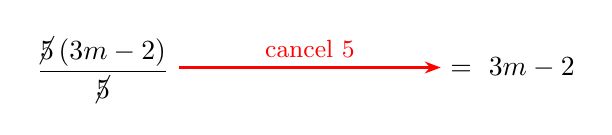
\begin{tikzpicture}[>={Stealth[length=2mm]}]
\node (f) {$\displaystyle \frac{\cancel{5}\,(3m-2)}{\cancel{5}}$};
\node (r) at (5.2,0) {$\displaystyle =\ 3m-2$};
\draw[->,red,thick] (f.east) -- (r.west) node[midway,above,font=\small]{cancel $5$};
\end{tikzpicture}
}
\end{center}
\small Cancellation diagram: factorise top and bottom, then strike the common factor.\normalsize

\medskip\hrule

\section*{Algebraic Fractions 9\quad\small\texttt{(a3-009)}}
\addcontentsline{toc}{section}{Algebraic Fractions 9 (a3-009)}
\textit{Difficulty: Foundation \quad\textbar\quad Marks: 3}

\question{Simplify fully: \( \frac{x^2 + 7x + 10}{x + 5} \)}

\textbf{Worked solution.}

\textit{Step 1: Factorise the quadratic expression in the numerator.}
\[\begin{gathered}
\frac{(x + 2)(x + 5)}{x + 5}
\end{gathered}\]
Find two numbers that multiply to make 10 and add to make 7. These are 2 and 5.

\textit{Step 2: Cancel the common binomial factor of \( (x + 5) \).}
\[\begin{gathered}
x + 2
\end{gathered}\]
Divide both the top and bottom by the shared bracket.

\begin{answerbox}
\textbf{Final answer:}\quad \(\displaystyle x + 2\)
\end{answerbox}
\textbf{Diagram.}

\begin{center}
\resizebox{\ifdim\width>\linewidth \linewidth\else \width\fi}{!}{%
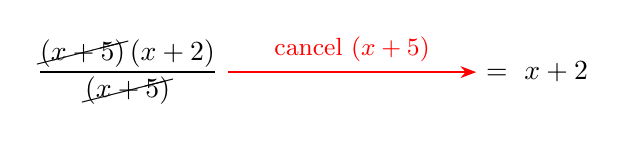
\begin{tikzpicture}[>={Stealth[length=2mm]}]
\node (f) {$\displaystyle \frac{\cancel{(x+5)}\,(x+2)}{\cancel{(x+5)}}$};
\node (r) at (5.2,0) {$\displaystyle =\ x+2$};
\draw[->,red,thick] (f.east) -- (r.west) node[midway,above,font=\small]{cancel $(x+5)$};
\end{tikzpicture}
}
\end{center}
\small Cancellation diagram: factorise top and bottom, then strike the common factor.\normalsize

\medskip\hrule

\section*{Algebraic Fractions 10\quad\small\texttt{(a3-010)}}
\addcontentsline{toc}{section}{Algebraic Fractions 10 (a3-010)}
\textit{Difficulty: Foundation \quad\textbar\quad Marks: 2}

\question{Simplify the expression: \( \frac{y^2 - 9}{y + 3} \)}

\textbf{Worked solution.}

\textit{Step 1: Recognise the numerator as a difference of two squares and factorise it.}
\[\begin{gathered}
\frac{(y - 3)(y + 3)}{y + 3}
\end{gathered}\]
\( y^2 \) and 9 are both square terms separated by a minus sign.

\textit{Step 2: Cancel the common factor \( (y + 3) \).}
\[\begin{gathered}
y - 3
\end{gathered}\]
The bracket \( (y + 3) \) appears on both the top and bottom, so they cancel out.

\begin{answerbox}
\textbf{Final answer:}\quad \(\displaystyle y - 3\)
\end{answerbox}
\textbf{Diagram.}

\begin{center}
\resizebox{\ifdim\width>\linewidth \linewidth\else \width\fi}{!}{%
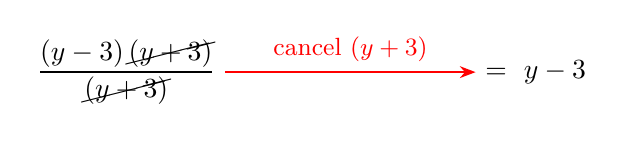
\begin{tikzpicture}[>={Stealth[length=2mm]}]
\node (f) {$\displaystyle \frac{(y-3)\,\cancel{(y+3)}}{\cancel{(y+3)}}$};
\node (r) at (5.2,0) {$\displaystyle =\ y-3$};
\draw[->,red,thick] (f.east) -- (r.west) node[midway,above,font=\small]{cancel $(y+3)$};
\end{tikzpicture}
}
\end{center}
\small Cancellation diagram: factorise top and bottom, then strike the common factor.\normalsize

\medskip\hrule

\section*{Algebraic Fractions 11\quad\small\texttt{(a3-011)}}
\addcontentsline{toc}{section}{Algebraic Fractions 11 (a3-011)}
\textit{Difficulty: Foundation \quad\textbar\quad Marks: 3}

\question{Simplify fully: \( \frac{8p^3q}{2pq^2} \)}

\textbf{Worked solution.}

\textit{Step 1: Divide the numerical coefficients.}
\[\begin{gathered}
\frac{4p^3q}{pq^2}
\end{gathered}\]
8 divided by 2 is 4.

\textit{Step 2: Use the laws of indices to simplify the \( p \) terms.}
\[\begin{gathered}
\frac{4p^2q}{q^2}
\end{gathered}\]
\( p^3 \div p^1 = p^{3-1} = p^2 \).

\textit{Step 3: Use the laws of indices to simplify the \( q \) terms.}
\[\begin{gathered}
\frac{4p^2}{q}
\end{gathered}\]
\( q^1 \div q^2 = q^{-1} \), which places a single \( q \) in the denominator.

\begin{answerbox}
\textbf{Final answer:}\quad \(\displaystyle \frac{4p^2}{q}\)
\end{answerbox}
\textbf{Diagram.}

\begin{center}
\resizebox{\ifdim\width>\linewidth \linewidth\else \width\fi}{!}{%
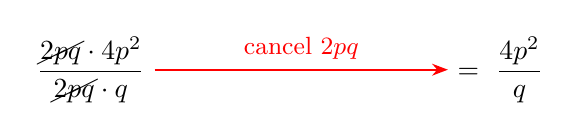
\begin{tikzpicture}[>={Stealth[length=2mm]}]
\node (f) {$\displaystyle \frac{\cancel{2pq}\cdot 4p^2}{\cancel{2pq}\cdot q}$};
\node (r) at (5.2,0) {$\displaystyle =\ \frac{4p^2}{q}$};
\draw[->,red,thick] (f.east) -- (r.west) node[midway,above,font=\small]{cancel $2pq$};
\end{tikzpicture}
}
\end{center}
\small Cancellation diagram: factorise top and bottom, then strike the common factor.\normalsize

\medskip\hrule

\section*{Algebraic Fractions 12\quad\small\texttt{(a3-012)}}
\addcontentsline{toc}{section}{Algebraic Fractions 12 (a3-012)}
\textit{Difficulty: Foundation \quad\textbar\quad Marks: 2}

\question{Write as a single fraction in its simplest form: \( \frac{3x}{4} + \frac{x}{4} \)}

\textbf{Worked solution.}

\textit{Step 1: Add the numerators together since the denominators are the same.}
\[\begin{gathered}
\frac{3x + x}{4}
\end{gathered}\]
When fractions have a common denominator, you can combine the top terms over the single denominator.

\textit{Step 2: Collect like terms on the numerator.}
\[\begin{gathered}
\frac{4x}{4}
\end{gathered}\]
\( 3x + 1x = 4x \).

\textit{Step 3: Simplify the fraction by cancelling the common factor of 4.}
\[\begin{gathered}
x
\end{gathered}\]
4 divided by 4 is 1, leaving just \( x \).

\begin{answerbox}
\textbf{Final answer:}\quad \(\displaystyle x\)
\end{answerbox}
\textbf{Diagram.}

\begin{center}
\resizebox{\ifdim\width>\linewidth \linewidth\else \width\fi}{!}{%
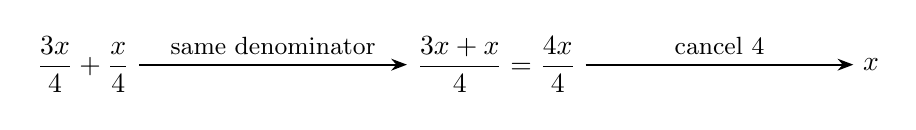
\begin{tikzpicture}[>={Stealth[length=2mm]},node distance=1.5cm and 3.4cm]
\node (s0) {$\displaystyle \frac{3x}{4}+\frac{x}{4}$};
\node (s1) [right=of s0] {$\displaystyle \frac{3x+x}{4}=\frac{4x}{4}$};
\node (s2) [right=of s1] {$\displaystyle x$};
\draw[->,thick] (s0) -- (s1) node[midway,above,font=\small]{same denominator};
\draw[->,thick] (s1) -- (s2) node[midway,above,font=\small]{cancel $4$};
\end{tikzpicture}
}
\end{center}
\small Solution flow: each arrow shows one operation taking the expression to the next form.\normalsize

\medskip\hrule

\section*{Algebraic Fractions 13\quad\small\texttt{(a3-013)}}
\addcontentsline{toc}{section}{Algebraic Fractions 13 (a3-013)}
\textit{Difficulty: Foundation \quad\textbar\quad Marks: 2}

\question{Express as a single fraction: \( \frac{x}{2} + \frac{x}{3} \)}

\textbf{Worked solution.}

\textit{Step 1: Find a common denominator for 2 and 3, which is 6.}
\[\begin{gathered}
\frac{3x}{6} + \frac{2x}{6}
\end{gathered}\]
Multiply the top and bottom of the first fraction by 3, and the top and bottom of the second fraction by 2.

\textit{Step 2: Add the numerators over the common denominator.}
\[\begin{gathered}
\frac{3x + 2x}{6}
\end{gathered}\]
Combine the terms now that the denominators match.

\textit{Step 3: Simplify the numerator.}
\[\begin{gathered}
\frac{5x}{6}
\end{gathered}\]
Collect the like terms: \( 3x + 2x = 5x \).

\begin{answerbox}
\textbf{Final answer:}\quad \(\displaystyle \frac{5x}{6}\)
\end{answerbox}
\textbf{Diagram.}

\begin{center}
\resizebox{\ifdim\width>\linewidth \linewidth\else \width\fi}{!}{%
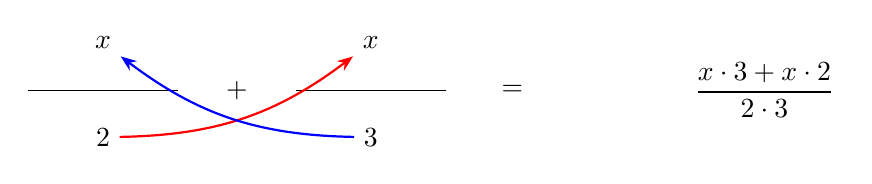
\begin{tikzpicture}[>={Stealth[length=2mm]}]
\node (a) at (0,0.6) {$x$};
\draw (-0.95,0) -- (0.95,0);
\node (b) at (0,-0.6) {$2$};
\node at (1.7,0) {$+$};
\node (c) at (3.4,0.6) {$x$};
\draw (2.45,0) -- (4.35,0);
\node (d) at (3.4,-0.6) {$3$};
\node at (5.2,0) {$=$};
\node at (8.4,0) {$\displaystyle \frac{x\cdot 3 + x\cdot 2}{2\cdot 3}$};
\draw[->,red,thick] (b) to[bend right=18] (c);
\draw[->,blue,thick] (d) to[bend left=18] (a);
\end{tikzpicture}
}
\end{center}
\small Cross-multiplication: each numerator multiplies the \emph{other} denominator (curved arrows); the denominators multiply to give the common denominator.\normalsize

\medskip\hrule

\section*{Algebraic Fractions 14\quad\small\texttt{(a3-014)}}
\addcontentsline{toc}{section}{Algebraic Fractions 14 (a3-014)}
\textit{Difficulty: Foundation \quad\textbar\quad Marks: 3}

\question{Simplify fully: \( \frac{2x^2 + 6x}{x^2 + 3x} \)}

\textbf{Worked solution.}

\textit{Step 1: Factorise the numerator by taking out the common factor of \( 2x \).}
\[\begin{gathered}
\frac{2x(x + 3)}{x^2 + 3x}
\end{gathered}\]
\( 2x \) is the highest common factor of both \( 2x^2 \) and \( 6x \).

\textit{Step 2: Factorise the denominator by taking out the common factor of \( x \).}
\[\begin{gathered}
\frac{2x(x + 3)}{x(x + 3)}
\end{gathered}\]
\( x \) is the highest common factor of both \( x^2 \) and \( 3x \).

\textit{Step 3: Cancel the common factors \( x \) and \( (x + 3) \) from the top and bottom.}
\[\begin{gathered}
2
\end{gathered}\]
Both the numerator and denominator share the algebraic factor \( x(x+3) \).

\begin{answerbox}
\textbf{Final answer:}\quad \(\displaystyle 2\)
\end{answerbox}
\textbf{Diagram.}

\begin{center}
\resizebox{\ifdim\width>\linewidth \linewidth\else \width\fi}{!}{%
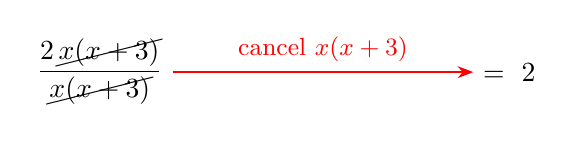
\begin{tikzpicture}[>={Stealth[length=2mm]}]
\node (f) {$\displaystyle \frac{2\,\cancel{x(x+3)}}{\cancel{x(x+3)}}$};
\node (r) at (5.2,0) {$\displaystyle =\ 2$};
\draw[->,red,thick] (f.east) -- (r.west) node[midway,above,font=\small]{cancel $x(x+3)$};
\end{tikzpicture}
}
\end{center}
\small Cancellation diagram: factorise top and bottom, then strike the common factor.\normalsize

\medskip\hrule

\section*{Algebraic Fractions 15\quad\small\texttt{(a3-015)}}
\addcontentsline{toc}{section}{Algebraic Fractions 15 (a3-015)}
\textit{Difficulty: Foundation \quad\textbar\quad Marks: 2}

\question{Simplify fully: \( \frac{2x}{3} \times \frac{5}{4x} \)}

\textbf{Worked solution.}

\textit{Step 1: Multiply the numerators together and the denominators together.}
\[\begin{gathered}
\frac{2x \times 5}{3 \times 4x}
\end{gathered}\]
When multiplying fractions, you multiply straight across the top and straight across the bottom.

\textit{Step 2: Simplify the resulting fraction.}
\[\begin{gathered}
\frac{10x}{12x}
\end{gathered}\]
Combine the terms to get a single numerator and denominator.

\textit{Step 3: Cancel the common factors from the top and bottom.}
\[\begin{gathered}
\frac{5}{6}
\end{gathered}\]
Divide both the top and bottom by 2 and cancel out the \( x \).

\begin{answerbox}
\textbf{Final answer:}\quad \(\displaystyle \frac{5}{6}\)
\end{answerbox}
\textbf{Diagram.}

\begin{center}
\resizebox{\ifdim\width>\linewidth \linewidth\else \width\fi}{!}{%
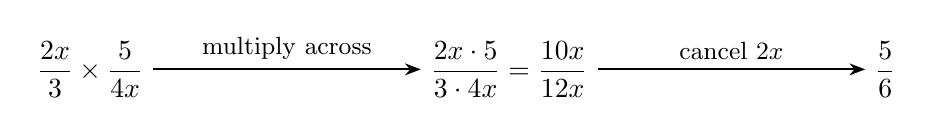
\begin{tikzpicture}[>={Stealth[length=2mm]},node distance=1.5cm and 3.4cm]
\node (s0) {$\displaystyle \frac{2x}{3}\times\frac{5}{4x}$};
\node (s1) [right=of s0] {$\displaystyle \frac{2x\cdot 5}{3\cdot 4x}=\frac{10x}{12x}$};
\node (s2) [right=of s1] {$\displaystyle \frac{5}{6}$};
\draw[->,thick] (s0) -- (s1) node[midway,above,font=\small]{multiply across};
\draw[->,thick] (s1) -- (s2) node[midway,above,font=\small]{cancel $2x$};
\end{tikzpicture}
}
\end{center}
\small Solution flow: each arrow shows one operation taking the expression to the next form.\normalsize

\medskip\hrule

\section*{Algebraic Fractions 16\quad\small\texttt{(a3-016)}}
\addcontentsline{toc}{section}{Algebraic Fractions 16 (a3-016)}
\textit{Difficulty: Foundation \quad\textbar\quad Marks: 3}

\question{Simplify fully: \( \frac{3a}{b} \div \frac{6a^2}{b^2} \)}

\textbf{Worked solution.}

\textit{Step 1: Change the division into a multiplication by flipping the second fraction.}
\[\begin{gathered}
\frac{3a}{b} \times \frac{b^2}{6a^2}
\end{gathered}\]
Use the rule: Keep the first fraction, Change the sign to multiply, Flip the second fraction.

\textit{Step 2: Multiply the numerators and the denominators.}
\[\begin{gathered}
\frac{3ab^2}{6a^2b}
\end{gathered}\]
Combine into a single algebraic fraction.

\textit{Step 3: Simplify the coefficients and use index laws to cancel the variables.}
\[\begin{gathered}
\frac{b}{2a}
\end{gathered}\]
\( \frac{3}{6} \) simplifies to \( \frac{1}{2} \). \( \frac{a}{a^2} \) leaves \( a \) on the bottom. \( \frac{b^2}{b} \) leaves \( b \) on the top.

\begin{answerbox}
\textbf{Final answer:}\quad \(\displaystyle \frac{b}{2a}\)
\end{answerbox}
\textbf{Diagram.}

\begin{center}
\resizebox{\ifdim\width>\linewidth \linewidth\else \width\fi}{!}{%
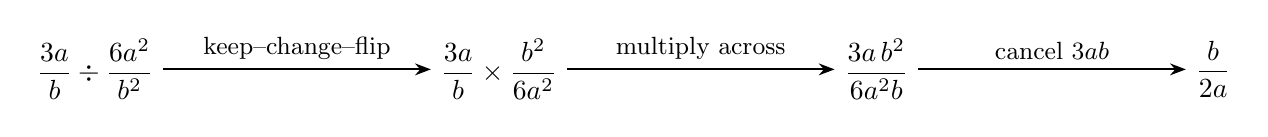
\begin{tikzpicture}[>={Stealth[length=2mm]},node distance=1.5cm and 3.4cm]
\node (s0) {$\displaystyle \frac{3a}{b}\div\frac{6a^2}{b^2}$};
\node (s1) [right=of s0] {$\displaystyle \frac{3a}{b}\times\frac{b^2}{6a^2}$};
\node (s2) [right=of s1] {$\displaystyle \frac{3a\,b^2}{6a^2 b}$};
\node (s3) [right=of s2] {$\displaystyle \frac{b}{2a}$};
\draw[->,thick] (s0) -- (s1) node[midway,above,font=\small]{keep--change--flip};
\draw[->,thick] (s1) -- (s2) node[midway,above,font=\small]{multiply across};
\draw[->,thick] (s2) -- (s3) node[midway,above,font=\small]{cancel $3ab$};
\end{tikzpicture}
}
\end{center}
\small Solution flow: each arrow shows one operation taking the expression to the next form.\normalsize

\medskip\hrule

\section*{Algebraic Fractions 17\quad\small\texttt{(a3-017)}}
\addcontentsline{toc}{section}{Algebraic Fractions 17 (a3-017)}
\textit{Difficulty: Foundation \quad\textbar\quad Marks: 3}

\question{Express as a single fraction in its simplest form: \( \frac{5}{x+1} - \frac{2}{x-2} \)}

\textbf{Worked solution.}

\textit{Step 1: Find a common denominator by multiplying the two denominators together.}
\[\begin{gathered}
\frac{5(x-2)}{(x+1)(x-2)} - \frac{2(x+1)}{(x+1)(x-2)}
\end{gathered}\]
Multiply the top and bottom of each fraction by the denominator of the other fraction.

\textit{Step 2: Combine the numerators over the single common denominator.}
\[\begin{gathered}
\frac{5(x-2) - 2(x+1)}{(x+1)(x-2)}
\end{gathered}\]
Now that the denominators are the same, subtract the second numerator from the first.

\textit{Step 3: Expand the brackets in the numerator and collect like terms.}
\[\begin{gathered}
\frac{5x - 10 - 2x - 2}{(x+1)(x-2)}
\end{gathered}\]
Be careful with the negative sign when expanding \( -2(x+1) \).

\textit{Step 4: Simplify the numerator to get the final answer.}
\[\begin{gathered}
\frac{3x - 12}{(x+1)(x-2)}
\end{gathered}\]
\( 5x - 2x = 3x \) and \( -10 - 2 = -12 \).

\begin{answerbox}
\textbf{Final answer:}\quad \(\displaystyle \frac{3x - 12}{(x+1)(x-2)}\)
\end{answerbox}
\textbf{Diagram.}

\begin{center}
\resizebox{\ifdim\width>\linewidth \linewidth\else \width\fi}{!}{%
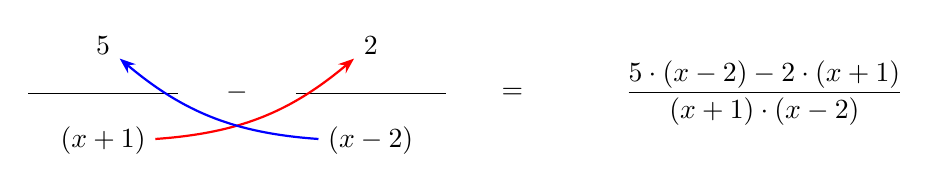
\begin{tikzpicture}[>={Stealth[length=2mm]}]
\node (a) at (0,0.6) {$5$};
\draw (-0.95,0) -- (0.95,0);
\node (b) at (0,-0.6) {$(x+1)$};
\node at (1.7,0) {$-$};
\node (c) at (3.4,0.6) {$2$};
\draw (2.45,0) -- (4.35,0);
\node (d) at (3.4,-0.6) {$(x-2)$};
\node at (5.2,0) {$=$};
\node at (8.4,0) {$\displaystyle \frac{5\cdot (x-2) - 2\cdot (x+1)}{(x+1)\cdot (x-2)}$};
\draw[->,red,thick] (b) to[bend right=18] (c);
\draw[->,blue,thick] (d) to[bend left=18] (a);
\end{tikzpicture}
}
\end{center}
\small Cross-multiplication: each numerator multiplies the \emph{other} denominator (curved arrows); the denominators multiply to give the common denominator.\normalsize

\medskip\hrule

\section*{Algebraic Fractions 18\quad\small\texttt{(a3-018)}}
\addcontentsline{toc}{section}{Algebraic Fractions 18 (a3-018)}
\textit{Difficulty: Foundation \quad\textbar\quad Marks: 4}

\question{Simplify fully: \( \frac{x^2 - x - 12}{x^2 - 16} \)}

\textbf{Worked solution.}

\textit{Step 1: Factorise the quadratic expression in the numerator.}
\[\begin{gathered}
\frac{(x - 4)(x + 3)}{x^2 - 16}
\end{gathered}\]
Find numbers that multiply to -12 and add to -1. These are -4 and 3.

\textit{Step 2: Factorise the denominator, which is a difference of two squares.}
\[\begin{gathered}
\frac{(x - 4)(x + 3)}{(x - 4)(x + 4)}
\end{gathered}\]
\( x^2 \) and 16 are both square terms, so it factorises to \( (x - 4)(x + 4) \).

\textit{Step 3: Cancel the common factor of \( (x - 4) \) from the numerator and denominator.}
\[\begin{gathered}
\frac{x + 3}{x + 4}
\end{gathered}\]
Divide the top and bottom by their shared bracket.

\begin{answerbox}
\textbf{Final answer:}\quad \(\displaystyle \frac{x + 3}{x + 4}\)
\end{answerbox}
\textbf{Diagram.}

\begin{center}
\resizebox{\ifdim\width>\linewidth \linewidth\else \width\fi}{!}{%
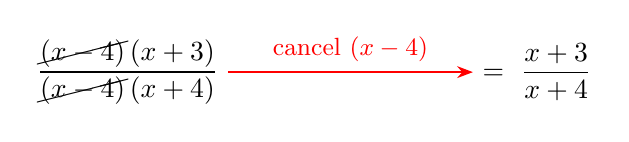
\begin{tikzpicture}[>={Stealth[length=2mm]}]
\node (f) {$\displaystyle \frac{\cancel{(x-4)}\,(x+3)}{\cancel{(x-4)}\,(x+4)}$};
\node (r) at (5.2,0) {$\displaystyle =\ \frac{x+3}{x+4}$};
\draw[->,red,thick] (f.east) -- (r.west) node[midway,above,font=\small]{cancel $(x-4)$};
\end{tikzpicture}
}
\end{center}
\small Cancellation diagram: factorise top and bottom, then strike the common factor.\normalsize

\medskip\hrule

\section*{Algebraic Fractions 19\quad\small\texttt{(a3-019)}}
\addcontentsline{toc}{section}{Algebraic Fractions 19 (a3-019)}
\textit{Difficulty: Foundation \quad\textbar\quad Marks: 2}

\question{Write as a single fraction: \( \frac{2}{x} + \frac{3}{2x} \)}

\textbf{Worked solution.}

\textit{Step 1: Identify the lowest common denominator, which is \( 2x \). Convert the first fraction.}
\[\begin{gathered}
\frac{4}{2x} + \frac{3}{2x}
\end{gathered}\]
Multiply the top and bottom of the first fraction by 2 so both fractions share the denominator \( 2x \).

\textit{Step 2: Add the numerators together.}
\[\begin{gathered}
\frac{4 + 3}{2x}
\end{gathered}\]
Since the denominators match, you can simply add the top values.

\textit{Step 3: Simplify to get the final fraction.}
\[\begin{gathered}
\frac{7}{2x}
\end{gathered}\]
Evaluate \( 4 + 3 \).

\begin{answerbox}
\textbf{Final answer:}\quad \(\displaystyle \frac{7}{2x}\)
\end{answerbox}
\textbf{Diagram.}

\begin{center}
\resizebox{\ifdim\width>\linewidth \linewidth\else \width\fi}{!}{%
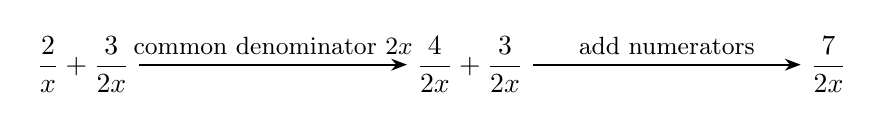
\begin{tikzpicture}[>={Stealth[length=2mm]},node distance=1.5cm and 3.4cm]
\node (s0) {$\displaystyle \frac{2}{x}+\frac{3}{2x}$};
\node (s1) [right=of s0] {$\displaystyle \frac{4}{2x}+\frac{3}{2x}$};
\node (s2) [right=of s1] {$\displaystyle \frac{7}{2x}$};
\draw[->,thick] (s0) -- (s1) node[midway,above,font=\small]{common denominator $2x$};
\draw[->,thick] (s1) -- (s2) node[midway,above,font=\small]{add numerators};
\end{tikzpicture}
}
\end{center}
\small Solution flow: each arrow shows one operation taking the expression to the next form.\normalsize

\medskip\hrule

\section*{Algebraic Fractions 20\quad\small\texttt{(a3-020)}}
\addcontentsline{toc}{section}{Algebraic Fractions 20 (a3-020)}
\textit{Difficulty: Foundation \quad\textbar\quad Marks: 3}

\question{Simplify fully: \( \frac{x+2}{3} \times \frac{9}{x^2 - 4} \)}

\textbf{Worked solution.}

\textit{Step 1: Factorise the expression \( x^2 - 4 \) in the denominator.}
\[\begin{gathered}
\frac{x+2}{3} \times \frac{9}{(x-2)(x+2)}
\end{gathered}\]
Recognise this as a difference of two squares.

\textit{Step 2: Cross-cancel the common numerical factors.}
\[\begin{gathered}
\frac{x+2}{1} \times \frac{3}{(x-2)(x+2)}
\end{gathered}\]
Divide the 9 on the top right and the 3 on the bottom left by 3.

\textit{Step 3: Cross-cancel the common algebraic factor \( (x+2) \).}
\[\begin{gathered}
1 \times \frac{3}{x-2}
\end{gathered}\]
The \( (x+2) \) on the top left cancels with the \( (x+2) \) on the bottom right.

\textit{Step 4: Multiply the remaining parts together.}
\[\begin{gathered}
\frac{3}{x-2}
\end{gathered}\]
Combine what is left after cancelling.

\begin{answerbox}
\textbf{Final answer:}\quad \(\displaystyle \frac{3}{x-2}\)
\end{answerbox}
\textbf{Diagram.}

\begin{center}
\resizebox{\ifdim\width>\linewidth \linewidth\else \width\fi}{!}{%
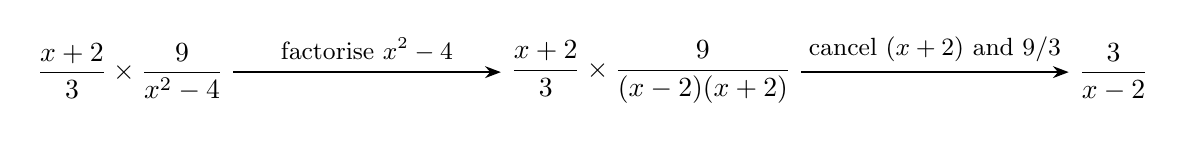
\begin{tikzpicture}[>={Stealth[length=2mm]},node distance=1.5cm and 3.4cm]
\node (s0) {$\displaystyle \frac{x+2}{3}\times\frac{9}{x^2-4}$};
\node (s1) [right=of s0] {$\displaystyle \frac{x+2}{3}\times\frac{9}{(x-2)(x+2)}$};
\node (s2) [right=of s1] {$\displaystyle \frac{3}{x-2}$};
\draw[->,thick] (s0) -- (s1) node[midway,above,font=\small]{factorise $x^2-4$};
\draw[->,thick] (s1) -- (s2) node[midway,above,font=\small]{cancel $(x+2)$ and $9/3$};
\end{tikzpicture}
}
\end{center}
\small Solution flow: each arrow shows one operation taking the expression to the next form.\normalsize

\medskip\hrule

\section*{Algebraic Fractions 21\quad\small\texttt{(a3-021)}}
\addcontentsline{toc}{section}{Algebraic Fractions 21 (a3-021)}
\textit{Difficulty: Foundation \quad\textbar\quad Marks: 3}

\question{Simplify fully: \( \frac{5 - x}{x^2 - 25} \)}

\textbf{Worked solution.}

\textit{Step 1: Factorise the denominator as a difference of two squares.}
\[\begin{gathered}
\frac{5 - x}{(x - 5)(x + 5)}
\end{gathered}\]
\( x^2 - 25 \) factorises to \( (x - 5)(x + 5) \).

\textit{Step 2: Factorise out a -1 from the numerator to reverse the terms.}
\[\begin{gathered}
\frac{-(x - 5)}{(x - 5)(x + 5)}
\end{gathered}\]
\( 5 - x \) is the exact negative of \( x - 5 \), so pulling out a -1 creates a matching bracket.

\textit{Step 3: Cancel the matching \( (x - 5) \) bracket.}
\[\begin{gathered}
\frac{-1}{x + 5}
\end{gathered}\]
Divide the top and bottom by \( (x - 5) \).

\begin{answerbox}
\textbf{Final answer:}\quad \(\displaystyle -\frac{1}{x + 5}\)
\end{answerbox}
\textbf{Diagram.}

\begin{center}
\resizebox{\ifdim\width>\linewidth \linewidth\else \width\fi}{!}{%
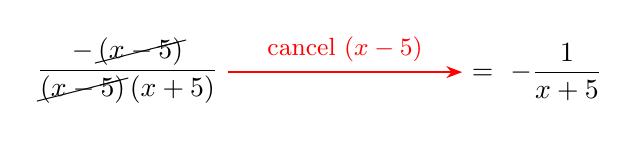
\begin{tikzpicture}[>={Stealth[length=2mm]}]
\node (f) {$\displaystyle \frac{-\,\cancel{(x-5)}}{\cancel{(x-5)}\,(x+5)}$};
\node (r) at (5.2,0) {$\displaystyle =\ -\frac{1}{x+5}$};
\draw[->,red,thick] (f.east) -- (r.west) node[midway,above,font=\small]{cancel $(x-5)$};
\end{tikzpicture}
}
\end{center}
\small Cancellation diagram: factorise top and bottom, then strike the common factor.\normalsize

\medskip\hrule

\section*{Algebraic Fractions 22\quad\small\texttt{(a3-022)}}
\addcontentsline{toc}{section}{Algebraic Fractions 22 (a3-022)}
\textit{Difficulty: Foundation \quad\textbar\quad Marks: 3}

\question{Express as a single fraction: \( \frac{2x - 1}{3} + \frac{x + 4}{5} \)}

\textbf{Worked solution.}

\textit{Step 1: Find a common denominator, which is 15.}
\[\begin{gathered}
\frac{5(2x - 1)}{15} + \frac{3(x + 4)}{15}
\end{gathered}\]
Multiply the top and bottom of the first fraction by 5, and the second by 3.

\textit{Step 2: Expand the brackets on the numerators and write over a single fraction.}
\[\begin{gathered}
\frac{10x - 5 + 3x + 12}{15}
\end{gathered}\]
Multiply the terms outside the brackets by the terms inside.

\textit{Step 3: Collect like terms on the numerator to simplify fully.}
\[\begin{gathered}
\frac{13x + 7}{15}
\end{gathered}\]
\( 10x + 3x = 13x \), and \( -5 + 12 = 7 \).

\begin{answerbox}
\textbf{Final answer:}\quad \(\displaystyle \frac{13x + 7}{15}\)
\end{answerbox}
\textbf{Diagram.}

\begin{center}
\resizebox{\ifdim\width>\linewidth \linewidth\else \width\fi}{!}{%
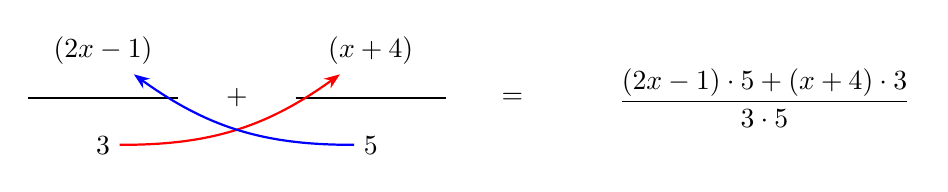
\begin{tikzpicture}[>={Stealth[length=2mm]}]
\node (a) at (0,0.6) {$(2x-1)$};
\draw (-0.95,0) -- (0.95,0);
\node (b) at (0,-0.6) {$3$};
\node at (1.7,0) {$+$};
\node (c) at (3.4,0.6) {$(x+4)$};
\draw (2.45,0) -- (4.35,0);
\node (d) at (3.4,-0.6) {$5$};
\node at (5.2,0) {$=$};
\node at (8.4,0) {$\displaystyle \frac{(2x-1)\cdot 5 + (x+4)\cdot 3}{3\cdot 5}$};
\draw[->,red,thick] (b) to[bend right=18] (c);
\draw[->,blue,thick] (d) to[bend left=18] (a);
\end{tikzpicture}
}
\end{center}
\small Cross-multiplication: each numerator multiplies the \emph{other} denominator (curved arrows); the denominators multiply to give the common denominator.\normalsize

\medskip\hrule

\section*{Algebraic Fractions 23\quad\small\texttt{(a3-023)}}
\addcontentsline{toc}{section}{Algebraic Fractions 23 (a3-023)}
\textit{Difficulty: Foundation \quad\textbar\quad Marks: 2}

\question{Simplify fully: \( \frac{2x+10}{6} \)}

\textbf{Worked solution.}

\textit{Step 1: Factorise the numerator by taking out the highest common factor of 2.}
\[\begin{gathered}
\frac{2(x+5)}{6}
\end{gathered}\]
Both 2x and 10 divide exactly by 2.

\textit{Step 2: Cancel the common factor from the top and bottom.}
\[\begin{gathered}
\frac{x+5}{3}
\end{gathered}\]
Divide the 2 on the top and the 6 on the bottom by 2.

\begin{answerbox}
\textbf{Final answer:}\quad \(\displaystyle \frac{x+5}{3}\)
\end{answerbox}
\textbf{Diagram.}

\begin{center}
\resizebox{\ifdim\width>\linewidth \linewidth\else \width\fi}{!}{%
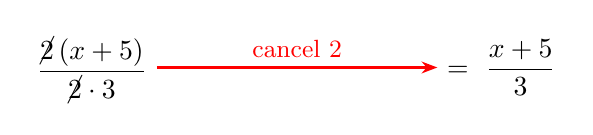
\begin{tikzpicture}[>={Stealth[length=2mm]}]
\node (f) {$\displaystyle \frac{\cancel{2}\,(x+5)}{\cancel{2}\cdot 3}$};
\node (r) at (5.2,0) {$\displaystyle =\ \frac{x+5}{3}$};
\draw[->,red,thick] (f.east) -- (r.west) node[midway,above,font=\small]{cancel $2$};
\end{tikzpicture}
}
\end{center}
\small Cancellation diagram: factorise top and bottom, then strike the common factor.\normalsize

\medskip\hrule

\section*{Algebraic Fractions 24\quad\small\texttt{(a3-024)}}
\addcontentsline{toc}{section}{Algebraic Fractions 24 (a3-024)}
\textit{Difficulty: Foundation \quad\textbar\quad Marks: 2}

\question{Simplify fully: \( \frac{6a-12b-15c}{3} \)}

\textbf{Worked solution.}

\textit{Step 1: Factorise the expression on the top line by finding the highest common numerical factor, which is 3.}
\[\begin{gathered}
\frac{3(2a-4b-5c)}{3}
\end{gathered}\]
3 divides exactly into 6a, -12b, and -15c.

\textit{Step 2: Cancel the common factor of 3 from the numerator and denominator.}
\[\begin{gathered}
2a-4b-5c
\end{gathered}\]
Dividing the top and bottom by 3 removes the fractional part entirely.

\begin{answerbox}
\textbf{Final answer:}\quad \(\displaystyle 2a-4b-5c\)
\end{answerbox}
\textbf{Diagram.}

\begin{center}
\resizebox{\ifdim\width>\linewidth \linewidth\else \width\fi}{!}{%
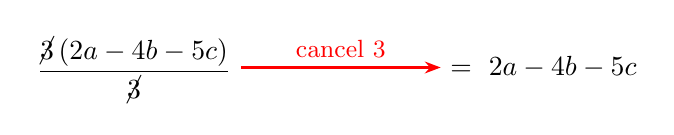
\begin{tikzpicture}[>={Stealth[length=2mm]}]
\node (f) {$\displaystyle \frac{\cancel{3}\,(2a-4b-5c)}{\cancel{3}}$};
\node (r) at (5.2,0) {$\displaystyle =\ 2a-4b-5c$};
\draw[->,red,thick] (f.east) -- (r.west) node[midway,above,font=\small]{cancel $3$};
\end{tikzpicture}
}
\end{center}
\small Cancellation diagram: factorise top and bottom, then strike the common factor.\normalsize

\medskip\hrule

\section*{Algebraic Fractions 25\quad\small\texttt{(a3-025)}}
\addcontentsline{toc}{section}{Algebraic Fractions 25 (a3-025)}
\textit{Difficulty: Foundation \quad\textbar\quad Marks: 3}

\question{Simplify fully: \( \frac{np^2-2n^2p}{np} \)}

\textbf{Worked solution.}

\textit{Step 1: Factorise the numerator by extracting the highest common algebraic factor, which is \( np \).}
\[\begin{gathered}
\frac{np(p-2n)}{np}
\end{gathered}\]
Both terms in the numerator share an \( n \) and a \( p \).

\textit{Step 2: Cancel the shared factor of \( np \) from the top and bottom.}
\[\begin{gathered}
p-2n
\end{gathered}\]
Dividing the top and bottom by \( np \) leaves just the bracketed expression.

\begin{answerbox}
\textbf{Final answer:}\quad \(\displaystyle p-2n\)
\end{answerbox}
\textbf{Diagram.}

\begin{center}
\resizebox{\ifdim\width>\linewidth \linewidth\else \width\fi}{!}{%
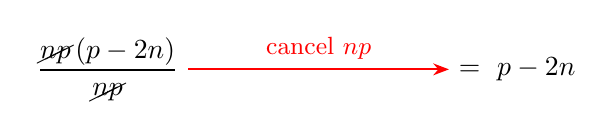
\begin{tikzpicture}[>={Stealth[length=2mm]}]
\node (f) {$\displaystyle \frac{\cancel{np}\,(p-2n)}{\cancel{np}}$};
\node (r) at (5.2,0) {$\displaystyle =\ p-2n$};
\draw[->,red,thick] (f.east) -- (r.west) node[midway,above,font=\small]{cancel $np$};
\end{tikzpicture}
}
\end{center}
\small Cancellation diagram: factorise top and bottom, then strike the common factor.\normalsize

\medskip\hrule

\section*{Algebraic Fractions 26\quad\small\texttt{(a3-026)}}
\addcontentsline{toc}{section}{Algebraic Fractions 26 (a3-026)}
\textit{Difficulty: Foundation \quad\textbar\quad Marks: 3}

\question{Express as a single fraction in its simplest form: \( \frac{5}{y-1} + \frac{3}{y-2} \)}

\textbf{Worked solution.}

\textit{Step 1: Find a common denominator by multiplying the two linear brackets together.}
\[\begin{gathered}
\frac{5(y-2)}{(y-1)(y-2)} + \frac{3(y-1)}{(y-1)(y-2)}
\end{gathered}\]
Multiply the top and bottom of each fraction by the denominator of the opposing fraction.

\textit{Step 2: Add the numerators together over the common denominator.}
\[\begin{gathered}
\frac{5(y-2) + 3(y-1)}{(y-1)(y-2)}
\end{gathered}\]
Combine the terms now that the denominators match.

\textit{Step 3: Expand the brackets on the numerator.}
\[\begin{gathered}
\frac{5y - 10 + 3y - 3}{(y-1)(y-2)}
\end{gathered}\]
Multiply the numbers outside the brackets by the terms inside.

\textit{Step 4: Collect like terms to fully simplify the numerator.}
\[\begin{gathered}
\frac{8y - 13}{(y-1)(y-2)}
\end{gathered}\]
\( 5y + 3y = 8y \) and \( -10 - 3 = -13 \).

\begin{answerbox}
\textbf{Final answer:}\quad \(\displaystyle \frac{8y - 13}{(y-1)(y-2)}\)
\end{answerbox}
\textbf{Diagram.}

\begin{center}
\resizebox{\ifdim\width>\linewidth \linewidth\else \width\fi}{!}{%
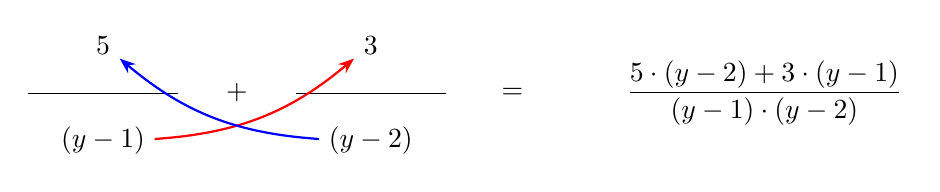
\begin{tikzpicture}[>={Stealth[length=2mm]}]
\node (a) at (0,0.6) {$5$};
\draw (-0.95,0) -- (0.95,0);
\node (b) at (0,-0.6) {$(y-1)$};
\node at (1.7,0) {$+$};
\node (c) at (3.4,0.6) {$3$};
\draw (2.45,0) -- (4.35,0);
\node (d) at (3.4,-0.6) {$(y-2)$};
\node at (5.2,0) {$=$};
\node at (8.4,0) {$\displaystyle \frac{5\cdot (y-2) + 3\cdot (y-1)}{(y-1)\cdot (y-2)}$};
\draw[->,red,thick] (b) to[bend right=18] (c);
\draw[->,blue,thick] (d) to[bend left=18] (a);
\end{tikzpicture}
}
\end{center}
\small Cross-multiplication: each numerator multiplies the \emph{other} denominator (curved arrows); the denominators multiply to give the common denominator.\normalsize

\medskip\hrule

\section*{Algebraic Fractions 27\quad\small\texttt{(a3-027)}}
\addcontentsline{toc}{section}{Algebraic Fractions 27 (a3-027)}
\textit{Difficulty: Foundation \quad\textbar\quad Marks: 3}

\question{Express as a single fraction in its simplest form: \( \frac{7}{r-5} - \frac{4}{r+3} \)}

\textbf{Worked solution.}

\textit{Step 1: Find a common denominator by multiplying the two denominators.}
\[\begin{gathered}
\frac{7(r+3)}{(r-5)(r+3)} - \frac{4(r-5)}{(r-5)(r+3)}
\end{gathered}\]
Cross-multiply the numerators and denominators to find equivalent fractions.

\textit{Step 2: Combine the numerators over the single denominator.}
\[\begin{gathered}
\frac{7(r+3) - 4(r-5)}{(r-5)(r+3)}
\end{gathered}\]
Subtract the second numerator from the first.

\textit{Step 3: Expand the brackets on the numerator carefully, paying attention to the negative sign.}
\[\begin{gathered}
\frac{7r + 21 - 4r + 20}{(r-5)(r+3)}
\end{gathered}\]
Be careful to note that \( -4 \times -5 = +20 \).

\textit{Step 4: Collect like terms on the numerator to finish.}
\[\begin{gathered}
\frac{3r + 41}{(r-5)(r+3)}
\end{gathered}\]
\( 7r - 4r = 3r \) and \( 21 + 20 = 41 \).

\begin{answerbox}
\textbf{Final answer:}\quad \(\displaystyle \frac{3r + 41}{(r-5)(r+3)}\)
\end{answerbox}
\textbf{Diagram.}

\begin{center}
\resizebox{\ifdim\width>\linewidth \linewidth\else \width\fi}{!}{%
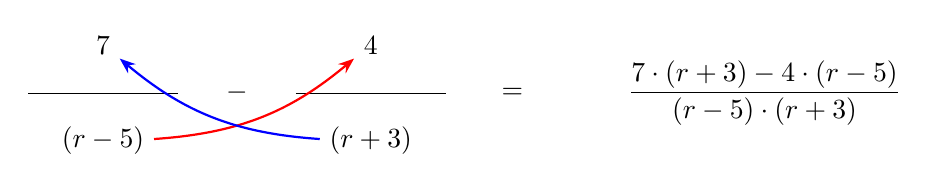
\begin{tikzpicture}[>={Stealth[length=2mm]}]
\node (a) at (0,0.6) {$7$};
\draw (-0.95,0) -- (0.95,0);
\node (b) at (0,-0.6) {$(r-5)$};
\node at (1.7,0) {$-$};
\node (c) at (3.4,0.6) {$4$};
\draw (2.45,0) -- (4.35,0);
\node (d) at (3.4,-0.6) {$(r+3)$};
\node at (5.2,0) {$=$};
\node at (8.4,0) {$\displaystyle \frac{7\cdot (r+3) - 4\cdot (r-5)}{(r-5)\cdot (r+3)}$};
\draw[->,red,thick] (b) to[bend right=18] (c);
\draw[->,blue,thick] (d) to[bend left=18] (a);
\end{tikzpicture}
}
\end{center}
\small Cross-multiplication: each numerator multiplies the \emph{other} denominator (curved arrows); the denominators multiply to give the common denominator.\normalsize

\medskip\hrule

\section*{Algebraic Fractions 28\quad\small\texttt{(a3-028)}}
\addcontentsline{toc}{section}{Algebraic Fractions 28 (a3-028)}
\textit{Difficulty: Foundation \quad\textbar\quad Marks: 4}

\question{Express as a single fraction in its simplest form: \( \frac{z+1}{z+2} - \frac{z+3}{z+4} \)}

\textbf{Worked solution.}

\textit{Step 1: Form equivalent fractions with a common denominator of \( (z+2)(z+4) \).}
\[\begin{gathered}
\frac{(z+1)(z+4)}{(z+2)(z+4)} - \frac{(z+3)(z+2)}{(z+2)(z+4)}
\end{gathered}\]
Multiply the top and bottom of each fraction by the opposing denominator.

\textit{Step 2: Write as a single fraction.}
\[\begin{gathered}
\frac{(z+1)(z+4) - (z+3)(z+2)}{(z+2)(z+4)}
\end{gathered}\]
Combine the numerators over the shared denominator.

\textit{Step 3: Expand the double brackets on the numerator.}
\[\begin{gathered}
\frac{(z^2 + 5z + 4) - (z^2 + 5z + 6)}{(z+2)(z+4)}
\end{gathered}\]
Multiply out each pair of brackets completely.

\textit{Step 4: Subtract the expanded terms and simplify the numerator.}
\[\begin{gathered}
\frac{-2}{(z+2)(z+4)}
\end{gathered}\]
\( z^2 - z^2 = 0 \), \( 5z - 5z = 0 \), and \( 4 - 6 = -2 \).

\begin{answerbox}
\textbf{Final answer:}\quad \(\displaystyle \frac{-2}{(z+2)(z+4)}\)
\end{answerbox}
\textbf{Diagram.}

\begin{center}
\resizebox{\ifdim\width>\linewidth \linewidth\else \width\fi}{!}{%
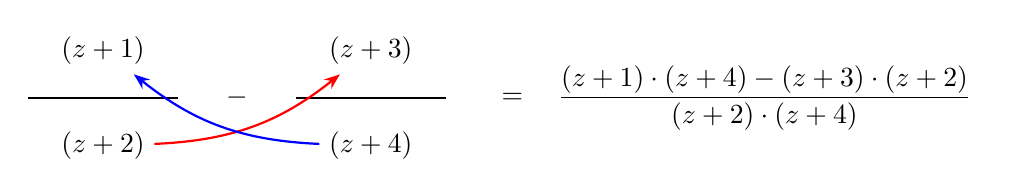
\begin{tikzpicture}[>={Stealth[length=2mm]}]
\node (a) at (0,0.6) {$(z+1)$};
\draw (-0.95,0) -- (0.95,0);
\node (b) at (0,-0.6) {$(z+2)$};
\node at (1.7,0) {$-$};
\node (c) at (3.4,0.6) {$(z+3)$};
\draw (2.45,0) -- (4.35,0);
\node (d) at (3.4,-0.6) {$(z+4)$};
\node at (5.2,0) {$=$};
\node at (8.4,0) {$\displaystyle \frac{(z+1)\cdot (z+4) - (z+3)\cdot (z+2)}{(z+2)\cdot (z+4)}$};
\draw[->,red,thick] (b) to[bend right=18] (c);
\draw[->,blue,thick] (d) to[bend left=18] (a);
\end{tikzpicture}
}
\end{center}
\small Cross-multiplication: each numerator multiplies the \emph{other} denominator (curved arrows); the denominators multiply to give the common denominator.\normalsize

\medskip\hrule

\section*{Algebraic Fractions 29\quad\small\texttt{(a3-029)}}
\addcontentsline{toc}{section}{Algebraic Fractions 29 (a3-029)}
\textit{Difficulty: Foundation \quad\textbar\quad Marks: 2}

\question{Express as a single fraction: \( \frac{2}{t} + \frac{13}{r^2} \)}

\textbf{Worked solution.}

\textit{Step 1: Identify the common denominator by multiplying the two distinct denominators together.}
\[\begin{gathered}
\frac{2(r^2)}{tr^2} + \frac{13(t)}{tr^2}
\end{gathered}\]
Multiply the first fraction by \( r^2 \) on the top and bottom, and the second fraction by \( t \) on the top and bottom.

\textit{Step 2: Combine the numerators over the single common denominator.}
\[\begin{gathered}
\frac{2r^2 + 13t}{tr^2}
\end{gathered}\]
Since the variables are different, you cannot collect the terms any further.

\begin{answerbox}
\textbf{Final answer:}\quad \(\displaystyle \frac{2r^2 + 13t}{tr^2}\)
\end{answerbox}
\textbf{Diagram.}

\begin{center}
\resizebox{\ifdim\width>\linewidth \linewidth\else \width\fi}{!}{%
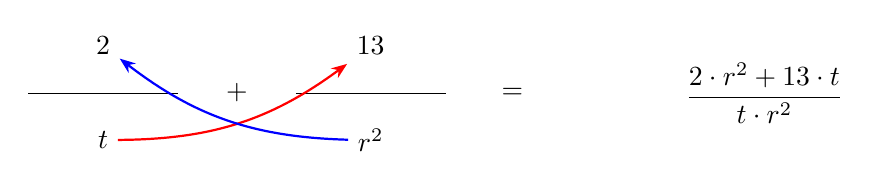
\begin{tikzpicture}[>={Stealth[length=2mm]}]
\node (a) at (0,0.6) {$2$};
\draw (-0.95,0) -- (0.95,0);
\node (b) at (0,-0.6) {$t$};
\node at (1.7,0) {$+$};
\node (c) at (3.4,0.6) {$13$};
\draw (2.45,0) -- (4.35,0);
\node (d) at (3.4,-0.6) {$r^2$};
\node at (5.2,0) {$=$};
\node at (8.4,0) {$\displaystyle \frac{2\cdot r^2 + 13\cdot t}{t\cdot r^2}$};
\draw[->,red,thick] (b) to[bend right=18] (c);
\draw[->,blue,thick] (d) to[bend left=18] (a);
\end{tikzpicture}
}
\end{center}
\small Cross-multiplication: each numerator multiplies the \emph{other} denominator (curved arrows); the denominators multiply to give the common denominator.\normalsize

\medskip\hrule

\section*{Algebraic Fractions 30\quad\small\texttt{(a3-030)}}
\addcontentsline{toc}{section}{Algebraic Fractions 30 (a3-030)}
\textit{Difficulty: Foundation \quad\textbar\quad Marks: 3}

\question{Express as a single fraction in its simplest form: \( \frac{8}{p} - \frac{1}{p-3} \)}

\textbf{Worked solution.}

\textit{Step 1: Find a common denominator, which is \( p(p-3) \).}
\[\begin{gathered}
\frac{8(p-3)}{p(p-3)} - \frac{1(p)}{p(p-3)}
\end{gathered}\]
Multiply the top and bottom of each fraction by the denominator of the other fraction.

\textit{Step 2: Combine the numerators over the single denominator.}
\[\begin{gathered}
\frac{8(p-3) - p}{p(p-3)}
\end{gathered}\]
Subtract the second numerator from the first.

\textit{Step 3: Expand the bracket on the numerator.}
\[\begin{gathered}
\frac{8p - 24 - p}{p(p-3)}
\end{gathered}\]
Multiply 8 by \( p \) and by \( -3 \).

\textit{Step 4: Collect like terms to simplify the numerator fully.}
\[\begin{gathered}
\frac{7p - 24}{p(p-3)}
\end{gathered}\]
\( 8p - 1p = 7p \).

\begin{answerbox}
\textbf{Final answer:}\quad \(\displaystyle \frac{7p - 24}{p(p-3)}\)
\end{answerbox}
\textbf{Diagram.}

\begin{center}
\resizebox{\ifdim\width>\linewidth \linewidth\else \width\fi}{!}{%
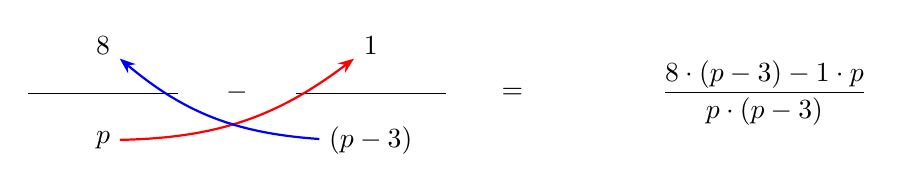
\begin{tikzpicture}[>={Stealth[length=2mm]}]
\node (a) at (0,0.6) {$8$};
\draw (-0.95,0) -- (0.95,0);
\node (b) at (0,-0.6) {$p$};
\node at (1.7,0) {$-$};
\node (c) at (3.4,0.6) {$1$};
\draw (2.45,0) -- (4.35,0);
\node (d) at (3.4,-0.6) {$(p-3)$};
\node at (5.2,0) {$=$};
\node at (8.4,0) {$\displaystyle \frac{8\cdot (p-3) - 1\cdot p}{p\cdot (p-3)}$};
\draw[->,red,thick] (b) to[bend right=18] (c);
\draw[->,blue,thick] (d) to[bend left=18] (a);
\end{tikzpicture}
}
\end{center}
\small Cross-multiplication: each numerator multiplies the \emph{other} denominator (curved arrows); the denominators multiply to give the common denominator.\normalsize

\medskip\hrule

\section*{Algebraic Fractions 31\quad\small\texttt{(a3-031)}}
\addcontentsline{toc}{section}{Algebraic Fractions 31 (a3-031)}
\textit{Difficulty: Foundation \quad\textbar\quad Marks: 3}

\question{Simplify fully: \( \frac{10yz - 40y^3z + 60y^2z^3}{10z^2} \)}

\textbf{Worked solution.}

\textit{Step 1: Factorise the numerator by extracting the highest common factor of all three terms, which is \( 10yz \).}
\[\begin{gathered}
\frac{10yz(1 - 4y^2 + 6yz^2)}{10z^2}
\end{gathered}\]
Look for the largest number and the highest powers of the variables that divide exactly into every term.

\textit{Step 2: Cancel the common factor of \( 10z \) from the numerator and denominator.}
\[\begin{gathered}
\frac{y(1 - 4y^2 + 6yz^2)}{z}
\end{gathered}\]
Divide the \( 10 \) on the top and bottom to get 1. Dividing \( z \) by \( z^2 \) leaves a single \( z \) on the denominator.

\begin{answerbox}
\textbf{Final answer:}\quad \(\displaystyle \frac{y(1 - 4y^2 + 6yz^2)}{z}\)
\end{answerbox}
\textbf{Diagram.}

\begin{center}
\resizebox{\ifdim\width>\linewidth \linewidth\else \width\fi}{!}{%
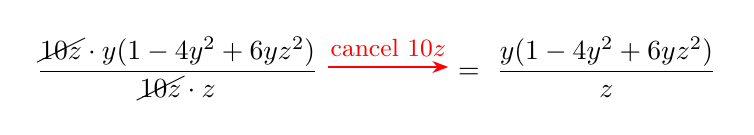
\begin{tikzpicture}[>={Stealth[length=2mm]}]
\node (f) {$\displaystyle \frac{\cancel{10z}\cdot y(1-4y^2+6yz^2)}{\cancel{10z}\cdot z}$};
\node (r) at (5.2,0) {$\displaystyle =\ \frac{y(1-4y^2+6yz^2)}{z}$};
\draw[->,red,thick] (f.east) -- (r.west) node[midway,above,font=\small]{cancel $10z$};
\end{tikzpicture}
}
\end{center}
\small Cancellation diagram: factorise top and bottom, then strike the common factor.\normalsize

\medskip\hrule

\section*{Algebraic Fractions 32\quad\small\texttt{(a3-032)}}
\addcontentsline{toc}{section}{Algebraic Fractions 32 (a3-032)}
\textit{Difficulty: Foundation \quad\textbar\quad Marks: 2}

\question{Simplify fully: \( \frac{4st + 6s^2t + 9s^3t}{2t} \)}

\textbf{Worked solution.}

\textit{Step 1: Factorise the numerator by extracting the common factor, which is \( t \).}
\[\begin{gathered}
\frac{t(4s + 6s^2 + 9s^3)}{2t}
\end{gathered}\]
There is no common numerical factor other than 1, but every term contains the variable \( t \).

\textit{Step 2: Cancel the common factor of \( t \) from the top and bottom.}
\[\begin{gathered}
\frac{4s + 6s^2 + 9s^3}{2}
\end{gathered}\]
Dividing the numerator and denominator by \( t \) removes it entirely.

\begin{answerbox}
\textbf{Final answer:}\quad \(\displaystyle \frac{4s + 6s^2 + 9s^3}{2}\)
\end{answerbox}
\textbf{Diagram.}

\begin{center}
\resizebox{\ifdim\width>\linewidth \linewidth\else \width\fi}{!}{%
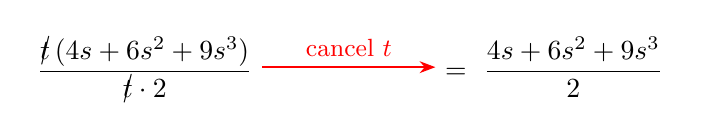
\begin{tikzpicture}[>={Stealth[length=2mm]}]
\node (f) {$\displaystyle \frac{\cancel{t}\,(4s+6s^2+9s^3)}{\cancel{t}\cdot 2}$};
\node (r) at (5.2,0) {$\displaystyle =\ \frac{4s+6s^2+9s^3}{2}$};
\draw[->,red,thick] (f.east) -- (r.west) node[midway,above,font=\small]{cancel $t$};
\end{tikzpicture}
}
\end{center}
\small Cancellation diagram: factorise top and bottom, then strike the common factor.\normalsize

\medskip\hrule

\section*{Algebraic Fractions 33\quad\small\texttt{(a3-033)}}
\addcontentsline{toc}{section}{Algebraic Fractions 33 (a3-033)}
\textit{Difficulty: Foundation \quad\textbar\quad Marks: 3}

\question{Express as a single fraction in its simplest form: \( \frac{1}{q+1} + \frac{3}{q-2} \)}

\textbf{Worked solution.}

\textit{Step 1: Find a common denominator by multiplying the two linear denominators together.}
\[\begin{gathered}
\frac{1(q-2)}{(q+1)(q-2)} + \frac{3(q+1)}{(q+1)(q-2)}
\end{gathered}\]
Multiply the top and bottom of each fraction by the opposing denominator.

\textit{Step 2: Combine the numerators over the single common denominator.}
\[\begin{gathered}
\frac{1(q-2) + 3(q+1)}{(q+1)(q-2)}
\end{gathered}\]
Add the terms together now that the denominators match.

\textit{Step 3: Expand the brackets on the numerator.}
\[\begin{gathered}
\frac{q - 2 + 3q + 3}{(q+1)(q-2)}
\end{gathered}\]
Multiply the terms outside the brackets by the terms inside.

\textit{Step 4: Collect like terms to fully simplify the numerator.}
\[\begin{gathered}
\frac{4q + 1}{(q+1)(q-2)}
\end{gathered}\]
\( q + 3q = 4q \) and \( -2 + 3 = 1 \).

\begin{answerbox}
\textbf{Final answer:}\quad \(\displaystyle \frac{4q + 1}{(q+1)(q-2)}\)
\end{answerbox}
\textbf{Diagram.}

\begin{center}
\resizebox{\ifdim\width>\linewidth \linewidth\else \width\fi}{!}{%
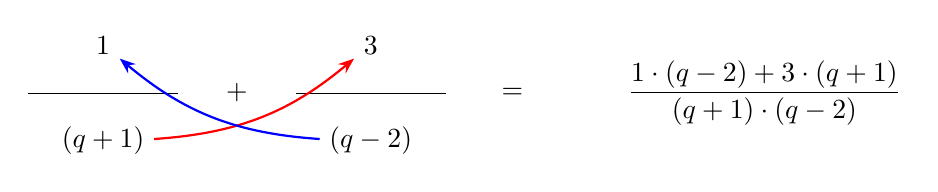
\begin{tikzpicture}[>={Stealth[length=2mm]}]
\node (a) at (0,0.6) {$1$};
\draw (-0.95,0) -- (0.95,0);
\node (b) at (0,-0.6) {$(q+1)$};
\node at (1.7,0) {$+$};
\node (c) at (3.4,0.6) {$3$};
\draw (2.45,0) -- (4.35,0);
\node (d) at (3.4,-0.6) {$(q-2)$};
\node at (5.2,0) {$=$};
\node at (8.4,0) {$\displaystyle \frac{1\cdot (q-2) + 3\cdot (q+1)}{(q+1)\cdot (q-2)}$};
\draw[->,red,thick] (b) to[bend right=18] (c);
\draw[->,blue,thick] (d) to[bend left=18] (a);
\end{tikzpicture}
}
\end{center}
\small Cross-multiplication: each numerator multiplies the \emph{other} denominator (curved arrows); the denominators multiply to give the common denominator.\normalsize

\medskip\hrule

\section*{Algebraic Fractions 34\quad\small\texttt{(a3-034)}}
\addcontentsline{toc}{section}{Algebraic Fractions 34 (a3-034)}
\textit{Difficulty: Foundation \quad\textbar\quad Marks: 3}

\question{Express as a single fraction in its simplest form: \( \frac{x}{x+z} + \frac{2z}{x-z} \)}

\textbf{Worked solution.}

\textit{Step 1: Form equivalent fractions with a common denominator of \( (x+z)(x-z) \).}
\[\begin{gathered}
\frac{x(x-z)}{(x+z)(x-z)} + \frac{2z(x+z)}{(x+z)(x-z)}
\end{gathered}\]
Multiply the first fraction by \( (x-z) \) top and bottom, and the second by \( (x+z) \).

\textit{Step 2: Combine the numerators over the shared denominator.}
\[\begin{gathered}
\frac{x(x-z) + 2z(x+z)}{(x+z)(x-z)}
\end{gathered}\]
Add the expanded numerators together.

\textit{Step 3: Expand the brackets on the numerator.}
\[\begin{gathered}
\frac{x^2 - xz + 2xz + 2z^2}{(x+z)(x-z)}
\end{gathered}\]
Multiply the outer variables into the brackets.

\textit{Step 4: Collect the like terms to simplify the numerator.}
\[\begin{gathered}
\frac{x^2 + xz + 2z^2}{(x+z)(x-z)}
\end{gathered}\]
\( -xz + 2xz = xz \).

\begin{answerbox}
\textbf{Final answer:}\quad \(\displaystyle \frac{x^2 + xz + 2z^2}{(x+z)(x-z)}\)
\end{answerbox}
\textbf{Diagram.}

\begin{center}
\resizebox{\ifdim\width>\linewidth \linewidth\else \width\fi}{!}{%
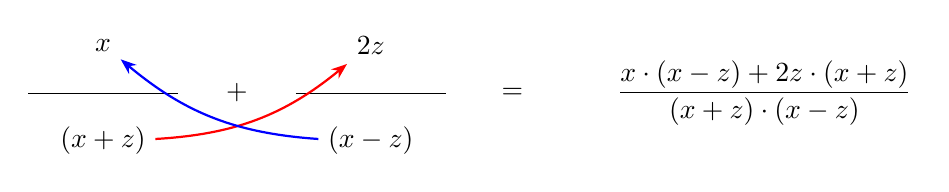
\begin{tikzpicture}[>={Stealth[length=2mm]}]
\node (a) at (0,0.6) {$x$};
\draw (-0.95,0) -- (0.95,0);
\node (b) at (0,-0.6) {$(x+z)$};
\node at (1.7,0) {$+$};
\node (c) at (3.4,0.6) {$2z$};
\draw (2.45,0) -- (4.35,0);
\node (d) at (3.4,-0.6) {$(x-z)$};
\node at (5.2,0) {$=$};
\node at (8.4,0) {$\displaystyle \frac{x\cdot (x-z) + 2z\cdot (x+z)}{(x+z)\cdot (x-z)}$};
\draw[->,red,thick] (b) to[bend right=18] (c);
\draw[->,blue,thick] (d) to[bend left=18] (a);
\end{tikzpicture}
}
\end{center}
\small Cross-multiplication: each numerator multiplies the \emph{other} denominator (curved arrows); the denominators multiply to give the common denominator.\normalsize

\medskip\hrule

\section*{Algebraic Fractions 35\quad\small\texttt{(a3-035)}}
\addcontentsline{toc}{section}{Algebraic Fractions 35 (a3-035)}
\textit{Difficulty: Foundation \quad\textbar\quad Marks: 2}

\question{Express as a single fraction: \( \frac{1}{2p} - \frac{1}{5q} \)}

\textbf{Worked solution.}

\textit{Step 1: Find a common denominator by multiplying the two distinct denominators, which gives \( 10pq \).}
\[\begin{gathered}
\frac{1(5q)}{10pq} - \frac{1(2p)}{10pq}
\end{gathered}\]
Multiply the first fraction by \( 5q \) top and bottom, and the second fraction by \( 2p \).

\textit{Step 2: Combine the numerators over the single common denominator.}
\[\begin{gathered}
\frac{5q - 2p}{10pq}
\end{gathered}\]
Subtract the numerators. These are not like terms, so they cannot be simplified further.

\begin{answerbox}
\textbf{Final answer:}\quad \(\displaystyle \frac{5q - 2p}{10pq}\)
\end{answerbox}
\textbf{Diagram.}

\begin{center}
\resizebox{\ifdim\width>\linewidth \linewidth\else \width\fi}{!}{%
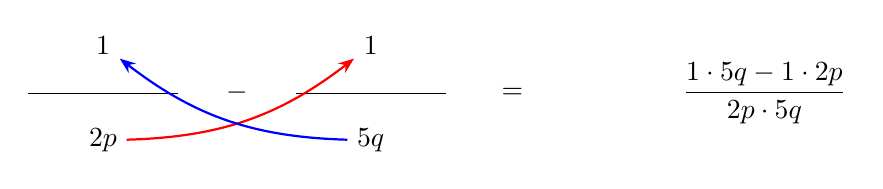
\begin{tikzpicture}[>={Stealth[length=2mm]}]
\node (a) at (0,0.6) {$1$};
\draw (-0.95,0) -- (0.95,0);
\node (b) at (0,-0.6) {$2p$};
\node at (1.7,0) {$-$};
\node (c) at (3.4,0.6) {$1$};
\draw (2.45,0) -- (4.35,0);
\node (d) at (3.4,-0.6) {$5q$};
\node at (5.2,0) {$=$};
\node at (8.4,0) {$\displaystyle \frac{1\cdot 5q - 1\cdot 2p}{2p\cdot 5q}$};
\draw[->,red,thick] (b) to[bend right=18] (c);
\draw[->,blue,thick] (d) to[bend left=18] (a);
\end{tikzpicture}
}
\end{center}
\small Cross-multiplication: each numerator multiplies the \emph{other} denominator (curved arrows); the denominators multiply to give the common denominator.\normalsize

\medskip\hrule

\section*{Algebraic Fractions 36\quad\small\texttt{(a3-036)}}
\addcontentsline{toc}{section}{Algebraic Fractions 36 (a3-036)}
\textit{Difficulty: Foundation \quad\textbar\quad Marks: 3}

\question{Express as a single fraction: \( \frac{2}{ab^3} - \frac{9}{a^3b} \)}

\textbf{Worked solution.}

\textit{Step 1: Identify the lowest common multiple for the denominators, which is \( a^3b^3 \).}
\[\begin{gathered}
\frac{2(a^2)}{ab^3(a^2)} - \frac{9(b^2)}{a^3b(b^2)}
\end{gathered}\]
To match the denominators, the first fraction needs an extra \( a^2 \) and the second fraction needs an extra \( b^2 \).

\textit{Step 2: Multiply the terms out.}
\[\begin{gathered}
\frac{2a^2}{a^3b^3} - \frac{9b^2}{a^3b^3}
\end{gathered}\]
Apply the adjustments to create equivalent fractions with matching bases.

\textit{Step 3: Combine the numerators over the single common denominator.}
\[\begin{gathered}
\frac{2a^2 - 9b^2}{a^3b^3}
\end{gathered}\]
Subtract the second numerator from the first.

\begin{answerbox}
\textbf{Final answer:}\quad \(\displaystyle \frac{2a^2 - 9b^2}{a^3b^3}\)
\end{answerbox}
\textbf{Diagram.}

\begin{center}
\resizebox{\ifdim\width>\linewidth \linewidth\else \width\fi}{!}{%
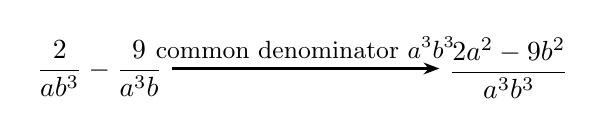
\begin{tikzpicture}[>={Stealth[length=2mm]},node distance=1.5cm and 3.4cm]
\node (s0) {$\displaystyle \frac{2}{ab^3}-\frac{9}{a^3b}$};
\node (s1) [right=of s0] {$\displaystyle \frac{2a^2-9b^2}{a^3b^3}$};
\draw[->,thick] (s0) -- (s1) node[midway,above,font=\small]{common denominator $a^3b^3$};
\end{tikzpicture}
}
\end{center}
\small Solution flow: each arrow shows one operation taking the expression to the next form.\normalsize

\medskip\hrule

\section*{Algebraic Fractions 37\quad\small\texttt{(a3-037)}}
\addcontentsline{toc}{section}{Algebraic Fractions 37 (a3-037)}
\textit{Difficulty: Foundation \quad\textbar\quad Marks: 4}

\question{Express as a single fraction in its simplest form: \( \frac{w}{2(w-2)} + \frac{3w}{w-7} \)}

\textbf{Worked solution.}

\textit{Step 1: Find a common denominator, which is \( 2(w-2)(w-7) \).}
\[\begin{gathered}
\frac{w(w-7)}{2(w-2)(w-7)} + \frac{3w(2)(w-2)}{2(w-2)(w-7)}
\end{gathered}\]
Multiply the top and bottom of the first fraction by \( (w-7) \), and the second fraction by \( 2(w-2) \).

\textit{Step 2: Combine the numerators and simplify the multiplier on the second term.}
\[\begin{gathered}
\frac{w(w-7) + 6w(w-2)}{2(w-2)(w-7)}
\end{gathered}\]
Note that \( 3w \times 2 = 6w \).

\textit{Step 3: Expand the brackets on the numerator.}
\[\begin{gathered}
\frac{w^2 - 7w + 6w^2 - 12w}{2(w-2)(w-7)}
\end{gathered}\]
Multiply the terms outside the brackets by the terms inside.

\textit{Step 4: Collect like terms to simplify the numerator fully.}
\[\begin{gathered}
\frac{7w^2 - 19w}{2(w-2)(w-7)}
\end{gathered}\]
\( w^2 + 6w^2 = 7w^2 \) and \( -7w - 12w = -19w \).

\begin{answerbox}
\textbf{Final answer:}\quad \(\displaystyle \frac{7w^2 - 19w}{2(w-2)(w-7)}\)
\end{answerbox}
\textbf{Diagram.}

\begin{center}
\resizebox{\ifdim\width>\linewidth \linewidth\else \width\fi}{!}{%
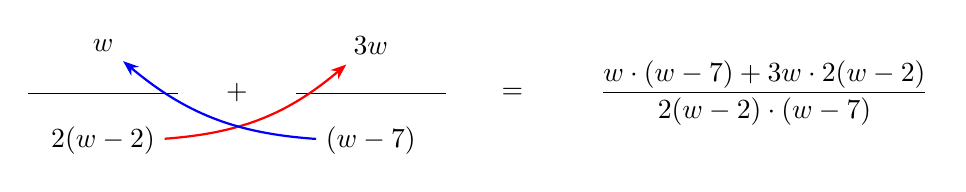
\begin{tikzpicture}[>={Stealth[length=2mm]}]
\node (a) at (0,0.6) {$w$};
\draw (-0.95,0) -- (0.95,0);
\node (b) at (0,-0.6) {$2(w-2)$};
\node at (1.7,0) {$+$};
\node (c) at (3.4,0.6) {$3w$};
\draw (2.45,0) -- (4.35,0);
\node (d) at (3.4,-0.6) {$(w-7)$};
\node at (5.2,0) {$=$};
\node at (8.4,0) {$\displaystyle \frac{w\cdot (w-7) + 3w\cdot 2(w-2)}{2(w-2)\cdot (w-7)}$};
\draw[->,red,thick] (b) to[bend right=18] (c);
\draw[->,blue,thick] (d) to[bend left=18] (a);
\end{tikzpicture}
}
\end{center}
\small Cross-multiplication: each numerator multiplies the \emph{other} denominator (curved arrows); the denominators multiply to give the common denominator.\normalsize

\medskip\hrule

\section*{Algebraic Fractions 38\quad\small\texttt{(a3-038)}}
\addcontentsline{toc}{section}{Algebraic Fractions 38 (a3-038)}
\textit{Difficulty: Foundation \quad\textbar\quad Marks: 3}

\question{Simplify fully: \( \frac{12cd - 6c^2d + 3c^3d^2}{12c^2de} \)}

\textbf{Worked solution.}

\textit{Step 1: Factorise the numerator by extracting the highest common factor of all three terms, which is \( 3cd \).}
\[\begin{gathered}
\frac{3cd(4 - 2c + c^2d)}{12c^2de}
\end{gathered}\]
3 is the largest number that divides into 12, 6, and 3. Each term also contains at least a \( c \) and a \( d \).

\textit{Step 2: Cancel the common factors of \( 3 \), \( c \), and \( d \) from the numerator and denominator.}
\[\begin{gathered}
\frac{4 - 2c + c^2d}{4ce}
\end{gathered}\]
Dividing 12 by 3 leaves 4 on the denominator. Dividing \( c^2 \) by \( c \) leaves \( c \), and the \( d \) is removed entirely.

\begin{answerbox}
\textbf{Final answer:}\quad \(\displaystyle \frac{4 - 2c + c^2d}{4ce}\)
\end{answerbox}
\textbf{Diagram.}

\begin{center}
\resizebox{\ifdim\width>\linewidth \linewidth\else \width\fi}{!}{%
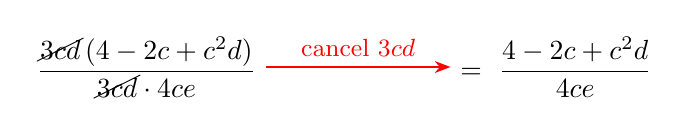
\begin{tikzpicture}[>={Stealth[length=2mm]}]
\node (f) {$\displaystyle \frac{\cancel{3cd}\,(4-2c+c^2d)}{\cancel{3cd}\cdot 4ce}$};
\node (r) at (5.2,0) {$\displaystyle =\ \frac{4-2c+c^2d}{4ce}$};
\draw[->,red,thick] (f.east) -- (r.west) node[midway,above,font=\small]{cancel $3cd$};
\end{tikzpicture}
}
\end{center}
\small Cancellation diagram: factorise top and bottom, then strike the common factor.\normalsize

\medskip\hrule

\section*{Algebraic Fractions 39\quad\small\texttt{(a3-039)}}
\addcontentsline{toc}{section}{Algebraic Fractions 39 (a3-039)}
\textit{Difficulty: Foundation \quad\textbar\quad Marks: 3}

\question{Express as a single fraction: \( \frac{2}{mn} - \frac{3m}{n} + \frac{n^2}{m} \)}

\textbf{Worked solution.}

\textit{Step 1: Identify the common denominator for all three fractions, which is \( mn \).}
\[\begin{gathered}
\frac{2}{mn} - \frac{3m(m)}{mn} + \frac{n^2(n)}{mn}
\end{gathered}\]
The first fraction already has the denominator \( mn \). Multiply the top and bottom of the second fraction by \( m \), and the third by \( n \).

\textit{Step 2: Simplify the numerators of the equivalent fractions.}
\[\begin{gathered}
\frac{2}{mn} - \frac{3m^2}{mn} + \frac{n^3}{mn}
\end{gathered}\]
Multiply the terms out: \( 3m \times m = 3m^2 \) and \( n^2 \times n = n^3 \).

\textit{Step 3: Combine the numerators over the single common denominator.}
\[\begin{gathered}
\frac{2 - 3m^2 + n^3}{mn}
\end{gathered}\]
Since these are not like terms, they cannot be simplified further.

\begin{answerbox}
\textbf{Final answer:}\quad \(\displaystyle \frac{2 - 3m^2 + n^3}{mn}\)
\end{answerbox}
\textbf{Diagram.}

\begin{center}
\resizebox{\ifdim\width>\linewidth \linewidth\else \width\fi}{!}{%
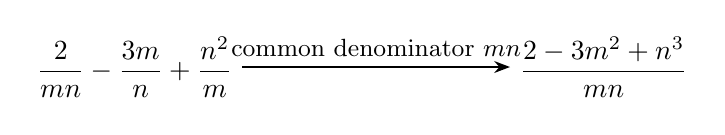
\begin{tikzpicture}[>={Stealth[length=2mm]},node distance=1.5cm and 3.4cm]
\node (s0) {$\displaystyle \frac{2}{mn}-\frac{3m}{n}+\frac{n^2}{m}$};
\node (s1) [right=of s0] {$\displaystyle \frac{2-3m^2+n^3}{mn}$};
\draw[->,thick] (s0) -- (s1) node[midway,above,font=\small]{common denominator $mn$};
\end{tikzpicture}
}
\end{center}
\small Solution flow: each arrow shows one operation taking the expression to the next form.\normalsize

\medskip\hrule

\section*{Algebraic Fractions 40\quad\small\texttt{(a3-040)}}
\addcontentsline{toc}{section}{Algebraic Fractions 40 (a3-040)}
\textit{Difficulty: Foundation \quad\textbar\quad Marks: 4}

\question{Express as a single fraction in its simplest form: \( \frac{y}{2x+3} - \frac{2y}{3-x} \)}

\textbf{Worked solution.}

\textit{Step 1: Find a common denominator by multiplying the two linear denominators together.}
\[\begin{gathered}
\frac{y(3-x)}{(2x+3)(3-x)} - \frac{2y(2x+3)}{(2x+3)(3-x)}
\end{gathered}\]
Multiply the top and bottom of each fraction by the opposing denominator.

\textit{Step 2: Combine the numerators over the single common denominator.}
\[\begin{gathered}
\frac{y(3-x) - 2y(2x+3)}{(2x+3)(3-x)}
\end{gathered}\]
Subtract the second numerator from the first.

\textit{Step 3: Expand the brackets on the numerator.}
\[\begin{gathered}
\frac{3y - xy - (4xy + 6y)}{(2x+3)(3-x)}
\end{gathered}\]
Multiply the terms outside the brackets by the terms inside. Be careful with the negative sign.

\textit{Step 4: Collect like terms and simplify fully.}
\[\begin{gathered}
\frac{-3y - 5xy}{(2x+3)(3-x)}
\end{gathered}\]
\( 3y - 6y = -3y \) and \( -xy - 4xy = -5xy \). You can also factorise out a \( -y \) on top to get \( \frac{-y(3+5x)}{(2x+3)(3-x)} \).

\begin{answerbox}
\textbf{Final answer:}\quad \(\displaystyle \frac{-3y - 5xy}{(2x+3)(3-x)}\)
\end{answerbox}
\textbf{Diagram.}

\begin{center}
\resizebox{\ifdim\width>\linewidth \linewidth\else \width\fi}{!}{%
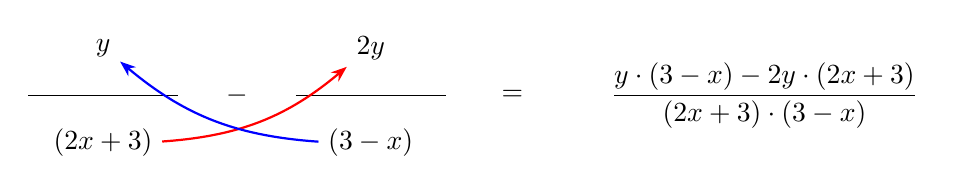
\begin{tikzpicture}[>={Stealth[length=2mm]}]
\node (a) at (0,0.6) {$y$};
\draw (-0.95,0) -- (0.95,0);
\node (b) at (0,-0.6) {$(2x+3)$};
\node at (1.7,0) {$-$};
\node (c) at (3.4,0.6) {$2y$};
\draw (2.45,0) -- (4.35,0);
\node (d) at (3.4,-0.6) {$(3-x)$};
\node at (5.2,0) {$=$};
\node at (8.4,0) {$\displaystyle \frac{y\cdot (3-x) - 2y\cdot (2x+3)}{(2x+3)\cdot (3-x)}$};
\draw[->,red,thick] (b) to[bend right=18] (c);
\draw[->,blue,thick] (d) to[bend left=18] (a);
\end{tikzpicture}
}
\end{center}
\small Cross-multiplication: each numerator multiplies the \emph{other} denominator (curved arrows); the denominators multiply to give the common denominator.\normalsize

\medskip\hrule

\section*{Algebraic Fractions 41\quad\small\texttt{(a3-041)}}
\addcontentsline{toc}{section}{Algebraic Fractions 41 (a3-041)}
\textit{Difficulty: Foundation \quad\textbar\quad Marks: 3}

\question{Express as a single fraction: \( \frac{1}{x} + \frac{2x}{y} + \frac{4}{x^2} \)}

\textbf{Worked solution.}

\textit{Step 1: Identify the lowest common multiple for the denominators, which is \( x^2y \).}
\[\begin{gathered}
\frac{1(xy)}{x^2y} + \frac{2x(x^2)}{x^2y} + \frac{4(y)}{x^2y}
\end{gathered}\]
Adjust each fraction so they all share the denominator \( x^2y \).

\textit{Step 2: Simplify the numerators of the equivalent fractions.}
\[\begin{gathered}
\frac{xy}{x^2y} + \frac{2x^3}{x^2y} + \frac{4y}{x^2y}
\end{gathered}\]
Multiply out the terms on the top of each fraction.

\textit{Step 3: Combine the numerators over the single common denominator.}
\[\begin{gathered}
\frac{xy + 2x^3 + 4y}{x^2y}
\end{gathered}\]
Add the terms together. They are not like terms, so the expression is complete.

\begin{answerbox}
\textbf{Final answer:}\quad \(\displaystyle \frac{xy + 2x^3 + 4y}{x^2y}\)
\end{answerbox}
\textbf{Diagram.}

\begin{center}
\resizebox{\ifdim\width>\linewidth \linewidth\else \width\fi}{!}{%
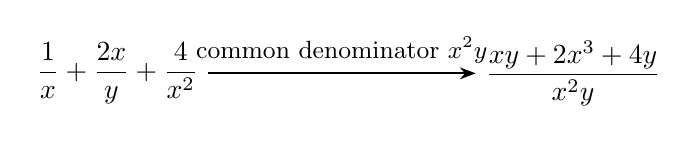
\begin{tikzpicture}[>={Stealth[length=2mm]},node distance=1.5cm and 3.4cm]
\node (s0) {$\displaystyle \frac{1}{x}+\frac{2x}{y}+\frac{4}{x^2}$};
\node (s1) [right=of s0] {$\displaystyle \frac{xy+2x^3+4y}{x^2y}$};
\draw[->,thick] (s0) -- (s1) node[midway,above,font=\small]{common denominator $x^2y$};
\end{tikzpicture}
}
\end{center}
\small Solution flow: each arrow shows one operation taking the expression to the next form.\normalsize

\medskip\hrule

\section*{Algebraic Fractions 42\quad\small\texttt{(a3-042)}}
\addcontentsline{toc}{section}{Algebraic Fractions 42 (a3-042)}
\textit{Difficulty: Foundation \quad\textbar\quad Marks: 3}

\question{Express as a single fraction: \( \frac{ab}{c} + \frac{bc}{a} + \frac{ca}{b} \)}

\textbf{Worked solution.}

\textit{Step 1: Find a common denominator by multiplying all three distinct denominators together to get \( abc \).}
\[\begin{gathered}
\frac{ab(ab)}{abc} + \frac{bc(bc)}{abc} + \frac{ca(ca)}{abc}
\end{gathered}\]
Multiply the top and bottom of each fraction by the variables it is missing from the common denominator.

\textit{Step 2: Simplify the numerators by applying the laws of indices.}
\[\begin{gathered}
\frac{a^2b^2}{abc} + \frac{b^2c^2}{abc} + \frac{c^2a^2}{abc}
\end{gathered}\]
For example, \( ab \times ab = a^2b^2 \).

\textit{Step 3: Combine the terms over the single denominator.}
\[\begin{gathered}
\frac{a^2b^2 + b^2c^2 + c^2a^2}{abc}
\end{gathered}\]
Add the numerators together.

\begin{answerbox}
\textbf{Final answer:}\quad \(\displaystyle \frac{a^2b^2 + b^2c^2 + c^2a^2}{abc}\)
\end{answerbox}
\textbf{Diagram.}

\begin{center}
\resizebox{\ifdim\width>\linewidth \linewidth\else \width\fi}{!}{%
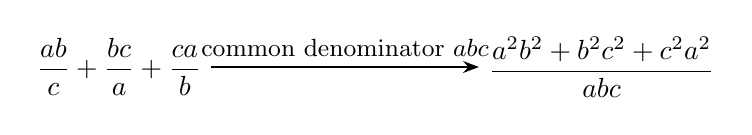
\begin{tikzpicture}[>={Stealth[length=2mm]},node distance=1.5cm and 3.4cm]
\node (s0) {$\displaystyle \frac{ab}{c}+\frac{bc}{a}+\frac{ca}{b}$};
\node (s1) [right=of s0] {$\displaystyle \frac{a^2b^2+b^2c^2+c^2a^2}{abc}$};
\draw[->,thick] (s0) -- (s1) node[midway,above,font=\small]{common denominator $abc$};
\end{tikzpicture}
}
\end{center}
\small Solution flow: each arrow shows one operation taking the expression to the next form.\normalsize

\medskip\hrule

\section*{Algebraic Fractions 43\quad\small\texttt{(a3-043)}}
\addcontentsline{toc}{section}{Algebraic Fractions 43 (a3-043)}
\textit{Difficulty: Foundation \quad\textbar\quad Marks: 3}

\question{Express as a single fraction: \( 2 + \frac{a^2}{b} - \frac{2b}{a^3} \)}

\textbf{Worked solution.}

\textit{Step 1: Identify the common denominator, which is \( a^3b \). Convert the whole number 2 into a fraction.}
\[\begin{gathered}
\frac{2(a^3b)}{a^3b} + \frac{a^2(a^3)}{a^3b} - \frac{2b(b)}{a^3b}
\end{gathered}\]
Adjust each term so they share the same denominator.

\textit{Step 2: Simplify the numerators of the equivalent fractions.}
\[\begin{gathered}
\frac{2a^3b}{a^3b} + \frac{a^5}{a^3b} - \frac{2b^2}{a^3b}
\end{gathered}\]
Multiply the terms out using index laws where necessary.

\textit{Step 3: Combine the numerators over the single common denominator.}
\[\begin{gathered}
\frac{2a^3b + a^5 - 2b^2}{a^3b}
\end{gathered}\]
Add and subtract the terms as written.

\begin{answerbox}
\textbf{Final answer:}\quad \(\displaystyle \frac{2a^3b + a^5 - 2b^2}{a^3b}\)
\end{answerbox}
\textbf{Diagram.}

\begin{center}
\resizebox{\ifdim\width>\linewidth \linewidth\else \width\fi}{!}{%
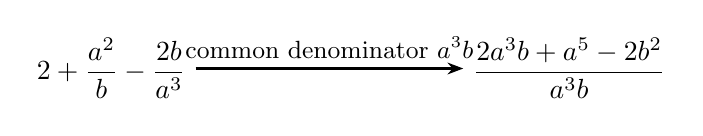
\begin{tikzpicture}[>={Stealth[length=2mm]},node distance=1.5cm and 3.4cm]
\node (s0) {$\displaystyle 2+\frac{a^2}{b}-\frac{2b}{a^3}$};
\node (s1) [right=of s0] {$\displaystyle \frac{2a^3b+a^5-2b^2}{a^3b}$};
\draw[->,thick] (s0) -- (s1) node[midway,above,font=\small]{common denominator $a^3b$};
\end{tikzpicture}
}
\end{center}
\small Solution flow: each arrow shows one operation taking the expression to the next form.\normalsize

\medskip\hrule

\section*{Algebraic Fractions 44\quad\small\texttt{(a3-044)}}
\addcontentsline{toc}{section}{Algebraic Fractions 44 (a3-044)}
\textit{Difficulty: Foundation \quad\textbar\quad Marks: 3}

\question{Simplify fully: \( \frac{2x + x^2y - x^2}{x^2 + 3x} \)}

\textbf{Worked solution.}

\textit{Step 1: Factorise the numerator by extracting the common factor of \( x \).}
\[\begin{gathered}
\frac{x(2 + xy - x)}{x^2 + 3x}
\end{gathered}\]
Every term on the top line contains at least one \( x \).

\textit{Step 2: Factorise the denominator by extracting the common factor of \( x \).}
\[\begin{gathered}
\frac{x(2 + xy - x)}{x(x + 3)}
\end{gathered}\]
This reveals a common factor on both the top and the bottom.

\textit{Step 3: Cancel the common factor of \( x \) to simplify fully.}
\[\begin{gathered}
\frac{2 + xy - x}{x + 3}
\end{gathered}\]
Divide the top and bottom by \( x \).

\begin{answerbox}
\textbf{Final answer:}\quad \(\displaystyle \frac{2 + xy - x}{x + 3}\)
\end{answerbox}
\textbf{Diagram.}

\begin{center}
\resizebox{\ifdim\width>\linewidth \linewidth\else \width\fi}{!}{%
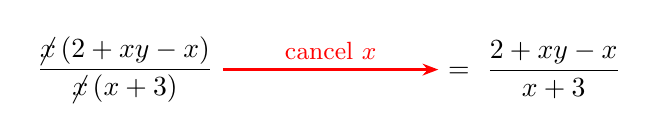
\begin{tikzpicture}[>={Stealth[length=2mm]}]
\node (f) {$\displaystyle \frac{\cancel{x}\,(2+xy-x)}{\cancel{x}\,(x+3)}$};
\node (r) at (5.2,0) {$\displaystyle =\ \frac{2+xy-x}{x+3}$};
\draw[->,red,thick] (f.east) -- (r.west) node[midway,above,font=\small]{cancel $x$};
\end{tikzpicture}
}
\end{center}
\small Cancellation diagram: factorise top and bottom, then strike the common factor.\normalsize

\medskip\hrule

\section*{Algebraic Fractions 45\quad\small\texttt{(a3-045)}}
\addcontentsline{toc}{section}{Algebraic Fractions 45 (a3-045)}
\textit{Difficulty: Foundation \quad\textbar\quad Marks: 3}

\question{Simplify fully: \( \frac{12cd - 6c^2d + 3c^3d^2}{12c^2de} \)}

\textbf{Worked solution.}

\textit{Step 1: Factorise the numerator by extracting the highest common factor of \( 3cd \).}
\[\begin{gathered}
\frac{3cd(4 - 2c + c^2d)}{12c^2de}
\end{gathered}\]
3 is the largest number that divides into 12, 6, and 3. Each term also contains at least a \( c \) and a \( d \).

\textit{Step 2: Cancel the common factors of \( 3 \), \( c \), and \( d \) from the numerator and denominator.}
\[\begin{gathered}
\frac{4 - 2c + c^2d}{4ce}
\end{gathered}\]
Dividing 12 by 3 leaves 4 on the denominator. Dividing \( c^2 \) by \( c \) leaves a single \( c \), and the \( d \) cancels entirely. The \( e \) is unaffected.

\begin{answerbox}
\textbf{Final answer:}\quad \(\displaystyle \frac{4 - 2c + c^2d}{4ce}\)
\end{answerbox}
\textbf{Diagram.}

\begin{center}
\resizebox{\ifdim\width>\linewidth \linewidth\else \width\fi}{!}{%
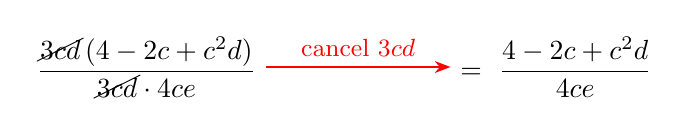
\begin{tikzpicture}[>={Stealth[length=2mm]}]
\node (f) {$\displaystyle \frac{\cancel{3cd}\,(4-2c+c^2d)}{\cancel{3cd}\cdot 4ce}$};
\node (r) at (5.2,0) {$\displaystyle =\ \frac{4-2c+c^2d}{4ce}$};
\draw[->,red,thick] (f.east) -- (r.west) node[midway,above,font=\small]{cancel $3cd$};
\end{tikzpicture}
}
\end{center}
\small Cancellation diagram: factorise top and bottom, then strike the common factor.\normalsize

\medskip\hrule

\section*{Algebraic Fractions 46\quad\small\texttt{(a3-046)}}
\addcontentsline{toc}{section}{Algebraic Fractions 46 (a3-046)}
\textit{Difficulty: Foundation \quad\textbar\quad Marks: 3}

\question{Simplify fully: \( \frac{x^2 - 9}{x^2 + 5x + 6} \)}

\textbf{Worked solution.}

\textit{Factorise the numerator and denominator separately, then cancel.}
\[\begin{gathered}
\begin{aligned} \frac{x^2 - 9}{x^2 + 5x + 6} &= \frac{(x-3)(x+3)}{(x+2)(x+3)} \\ &= \frac{x-3}{x+2} \end{aligned}
\end{gathered}\]
The numerator is a difference of two squares. The denominator factorises as a quadratic. Cancel the common factor \((x+3)\).

\begin{answerbox}
\textbf{Final answer:}\quad \(\displaystyle \frac{x-3}{x+2}\)
\end{answerbox}
\textbf{Diagram.}

\begin{center}
\resizebox{\ifdim\width>\linewidth \linewidth\else \width\fi}{!}{%
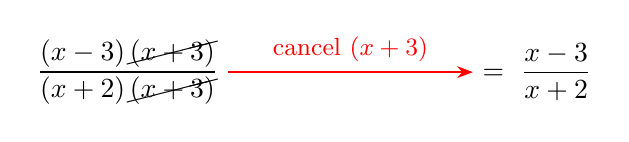
\begin{tikzpicture}[>={Stealth[length=2mm]}]
\node (f) {$\displaystyle \frac{(x-3)\,\cancel{(x+3)}}{(x+2)\,\cancel{(x+3)}}$};
\node (r) at (5.2,0) {$\displaystyle =\ \frac{x-3}{x+2}$};
\draw[->,red,thick] (f.east) -- (r.west) node[midway,above,font=\small]{cancel $(x+3)$};
\end{tikzpicture}
}
\end{center}
\small Cancellation diagram: factorise top and bottom, then strike the common factor.\normalsize

\medskip\hrule

\section*{Algebraic Fractions 47\quad\small\texttt{(a3-047)}}
\addcontentsline{toc}{section}{Algebraic Fractions 47 (a3-047)}
\textit{Difficulty: Foundation \quad\textbar\quad Marks: 2}

\question{Simplify fully: \( \frac{ax+ay}{az} \)}

\textbf{Worked solution.}

\textit{Step 1: Factorise the top line by taking out the common factor of \( a \).}
\[\begin{gathered}
\frac{a(x+y)}{az}
\end{gathered}\]
Both terms in the numerator share the variable \( a \).

\textit{Step 2: Cancel the common factor of \( a \) from the numerator and denominator.}
\[\begin{gathered}
\frac{x+y}{z}
\end{gathered}\]
Dividing the top and bottom by \( a \) simplifies the fraction.

\begin{answerbox}
\textbf{Final answer:}\quad \(\displaystyle \frac{x+y}{z}\)
\end{answerbox}
\textbf{Diagram.}

\begin{center}
\resizebox{\ifdim\width>\linewidth \linewidth\else \width\fi}{!}{%
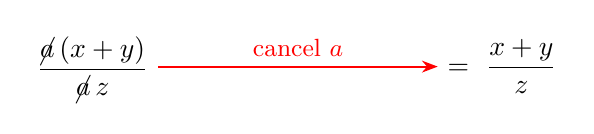
\begin{tikzpicture}[>={Stealth[length=2mm]}]
\node (f) {$\displaystyle \frac{\cancel{a}\,(x+y)}{\cancel{a}\,z}$};
\node (r) at (5.2,0) {$\displaystyle =\ \frac{x+y}{z}$};
\draw[->,red,thick] (f.east) -- (r.west) node[midway,above,font=\small]{cancel $a$};
\end{tikzpicture}
}
\end{center}
\small Cancellation diagram: factorise top and bottom, then strike the common factor.\normalsize

\medskip\hrule

\section*{Algebraic Fractions 48\quad\small\texttt{(a3-048)}}
\addcontentsline{toc}{section}{Algebraic Fractions 48 (a3-048)}
\textit{Difficulty: Foundation \quad\textbar\quad Marks: 2}

\question{Express as a single fraction: \( \frac{x}{3} + \frac{x}{4} \)}

\textbf{Worked solution.}

\textit{Step 1: Find a common denominator for 3 and 4, which is 12.}
\[\begin{gathered}
\frac{4x}{12} + \frac{3x}{12}
\end{gathered}\]
Multiply the top and bottom of the first fraction by 4, and the top and bottom of the second fraction by 3.

\textit{Step 2: Add the numerators together over the common denominator.}
\[\begin{gathered}
\frac{4x + 3x}{12}
\end{gathered}\]
Combine the terms now that the denominators match.

\textit{Step 3: Simplify the numerator.}
\[\begin{gathered}
\frac{7x}{12}
\end{gathered}\]
Collect the like terms: \( 4x + 3x = 7x \).

\begin{answerbox}
\textbf{Final answer:}\quad \(\displaystyle \frac{7x}{12}\)
\end{answerbox}
\textbf{Diagram.}

\begin{center}
\resizebox{\ifdim\width>\linewidth \linewidth\else \width\fi}{!}{%
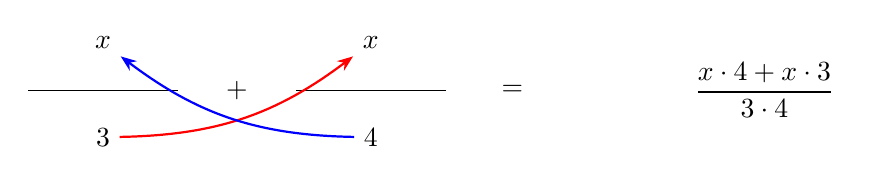
\begin{tikzpicture}[>={Stealth[length=2mm]}]
\node (a) at (0,0.6) {$x$};
\draw (-0.95,0) -- (0.95,0);
\node (b) at (0,-0.6) {$3$};
\node at (1.7,0) {$+$};
\node (c) at (3.4,0.6) {$x$};
\draw (2.45,0) -- (4.35,0);
\node (d) at (3.4,-0.6) {$4$};
\node at (5.2,0) {$=$};
\node at (8.4,0) {$\displaystyle \frac{x\cdot 4 + x\cdot 3}{3\cdot 4}$};
\draw[->,red,thick] (b) to[bend right=18] (c);
\draw[->,blue,thick] (d) to[bend left=18] (a);
\end{tikzpicture}
}
\end{center}
\small Cross-multiplication: each numerator multiplies the \emph{other} denominator (curved arrows); the denominators multiply to give the common denominator.\normalsize

\medskip\hrule

\section*{Algebraic Fractions 49\quad\small\texttt{(a3-049)}}
\addcontentsline{toc}{section}{Algebraic Fractions 49 (a3-049)}
\textit{Difficulty: Foundation \quad\textbar\quad Marks: 2}

\question{Simplify fully: \( \frac{5x^2 + 10xy}{5x} \)}

\textbf{Worked solution.}

\textit{Step 1: Factorise the numerator by extracting the highest common factor, which is \( 5x \).}
\[\begin{gathered}
\frac{5x(x + 2y)}{5x}
\end{gathered}\]
Look for the largest number and the highest power of the variables that divide exactly into both terms on the top.

\textit{Step 2: Cancel the common factor of \( 5x \) from the numerator and the denominator.}
\[\begin{gathered}
x + 2y
\end{gathered}\]
Dividing the top and bottom by \( 5x \) removes the fraction entirely.

\begin{answerbox}
\textbf{Final answer:}\quad \(\displaystyle x + 2y\)
\end{answerbox}
\textbf{Diagram.}

\begin{center}
\resizebox{\ifdim\width>\linewidth \linewidth\else \width\fi}{!}{%
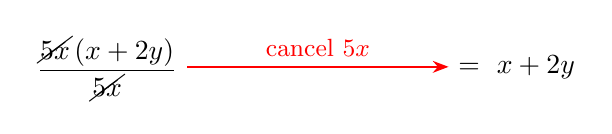
\begin{tikzpicture}[>={Stealth[length=2mm]}]
\node (f) {$\displaystyle \frac{\cancel{5x}\,(x+2y)}{\cancel{5x}}$};
\node (r) at (5.2,0) {$\displaystyle =\ x+2y$};
\draw[->,red,thick] (f.east) -- (r.west) node[midway,above,font=\small]{cancel $5x$};
\end{tikzpicture}
}
\end{center}
\small Cancellation diagram: factorise top and bottom, then strike the common factor.\normalsize

\medskip\hrule

\section*{Algebraic Fractions 50\quad\small\texttt{(a3-050)}}
\addcontentsline{toc}{section}{Algebraic Fractions 50 (a3-050)}
\textit{Difficulty: Foundation \quad\textbar\quad Marks: 3}

\question{Express as a single fraction in its simplest form: \( \frac{2}{x+3} - \frac{1}{x-1} \)}

\textbf{Worked solution.}

\textit{Step 1: Find a common denominator by multiplying the two linear denominators together.}
\[\begin{gathered}
\frac{2(x-1)}{(x+3)(x-1)} - \frac{1(x+3)}{(x+3)(x-1)}
\end{gathered}\]
Multiply the top and bottom of each fraction by the denominator of the other fraction.

\textit{Step 2: Combine the numerators over the single common denominator.}
\[\begin{gathered}
\frac{2(x-1) - 1(x+3)}{(x+3)(x-1)}
\end{gathered}\]
Subtract the second numerator from the first now that the denominators match.

\textit{Step 3: Expand the brackets on the numerator.}
\[\begin{gathered}
\frac{2x - 2 - x - 3}{(x+3)(x-1)}
\end{gathered}\]
Be careful with the negative sign when expanding the second bracket.

\textit{Step 4: Collect like terms to fully simplify the numerator.}
\[\begin{gathered}
\frac{x - 5}{(x+3)(x-1)}
\end{gathered}\]
\( 2x - x = x \) and \( -2 - 3 = -5 \).

\begin{answerbox}
\textbf{Final answer:}\quad \(\displaystyle \frac{x - 5}{(x+3)(x-1)}\)
\end{answerbox}
\textbf{Diagram.}

\begin{center}
\resizebox{\ifdim\width>\linewidth \linewidth\else \width\fi}{!}{%
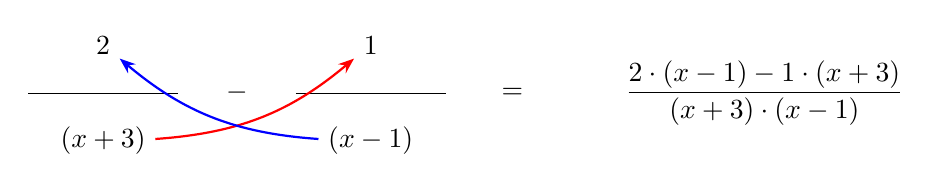
\begin{tikzpicture}[>={Stealth[length=2mm]}]
\node (a) at (0,0.6) {$2$};
\draw (-0.95,0) -- (0.95,0);
\node (b) at (0,-0.6) {$(x+3)$};
\node at (1.7,0) {$-$};
\node (c) at (3.4,0.6) {$1$};
\draw (2.45,0) -- (4.35,0);
\node (d) at (3.4,-0.6) {$(x-1)$};
\node at (5.2,0) {$=$};
\node at (8.4,0) {$\displaystyle \frac{2\cdot (x-1) - 1\cdot (x+3)}{(x+3)\cdot (x-1)}$};
\draw[->,red,thick] (b) to[bend right=18] (c);
\draw[->,blue,thick] (d) to[bend left=18] (a);
\end{tikzpicture}
}
\end{center}
\small Cross-multiplication: each numerator multiplies the \emph{other} denominator (curved arrows); the denominators multiply to give the common denominator.\normalsize

\medskip\hrule

\section*{Algebraic Fractions 51\quad\small\texttt{(a3-051)}}
\addcontentsline{toc}{section}{Algebraic Fractions 51 (a3-051)}
\textit{Difficulty: Foundation \quad\textbar\quad Marks: 3}

\question{Express as a single fraction: \( 3 + \frac{2}{x-2} \)}

\textbf{Worked solution.}

\textit{Step 1: Rewrite the whole number 3 as a fraction with a denominator of \( x-2 \).}
\[\begin{gathered}
\frac{3(x-2)}{x-2} + \frac{2}{x-2}
\end{gathered}\]
Multiply the whole number by \( \frac{x-2}{x-2} \) so it shares the same base as the fraction.

\textit{Step 2: Expand the numerator of the first fraction.}
\[\begin{gathered}
\frac{3x - 6}{x-2} + \frac{2}{x-2}
\end{gathered}\]
Multiply the 3 into the bracket.

\textit{Step 3: Add the numerators together over the common denominator and simplify.}
\[\begin{gathered}
\frac{3x - 6 + 2}{x-2}
\end{gathered}\]
Combine the constants: \( -6 + 2 = -4 \).

\begin{answerbox}
\textbf{Final answer:}\quad \(\displaystyle \frac{3x - 4}{x-2}\)
\end{answerbox}
\textbf{Diagram.}

\begin{center}
\resizebox{\ifdim\width>\linewidth \linewidth\else \width\fi}{!}{%
\begin{tikzpicture}[>={Stealth[length=2mm]},node distance=1.5cm and 3.4cm]
\node (s0) {$\displaystyle 3+\frac{2}{x-2}$};
\node (s1) [right=of s0] {$\displaystyle \frac{3(x-2)+2}{x-2}$};
\node (s2) [right=of s1] {$\displaystyle \frac{3x-4}{x-2}$};
\draw[->,thick] (s0) -- (s1) node[midway,above,font=\small]{write $3=\tfrac{3(x-2)}{x-2}$};
\draw[->,thick] (s1) -- (s2) node[midway,above,font=\small]{simplify};
\end{tikzpicture}
}
\end{center}
\small Solution flow: each arrow shows one operation taking the expression to the next form.\normalsize

\medskip\hrule

\section*{Algebraic Fractions 52\quad\small\texttt{(a3-052)}}
\addcontentsline{toc}{section}{Algebraic Fractions 52 (a3-052)}
\textit{Difficulty: Foundation \quad\textbar\quad Marks: 3}

\question{Simplify fully: \( \frac{x^2 - 16}{4x + 16} \)}

\textbf{Worked solution.}

\textit{Step 1: Factorise the numerator using the difference of two squares.}
\[\begin{gathered}
\frac{(x-4)(x+4)}{4x + 16}
\end{gathered}\]
\( x^2 \) and 16 are both square terms separated by a subtraction sign.

\textit{Step 2: Factorise the denominator by extracting the common numerical factor of 4.}
\[\begin{gathered}
\frac{(x-4)(x+4)}{4(x+4)}
\end{gathered}\]
This reveals a common binomial bracket on the top and bottom.

\textit{Step 3: Cancel the common factor of \( (x+4) \) from the numerator and denominator.}
\[\begin{gathered}
\frac{x-4}{4}
\end{gathered}\]
Divide the top and bottom by the shared bracket to leave the final simplified fraction.

\begin{answerbox}
\textbf{Final answer:}\quad \(\displaystyle \frac{x-4}{4}\)
\end{answerbox}
\textbf{Diagram.}

\begin{center}
\resizebox{\ifdim\width>\linewidth \linewidth\else \width\fi}{!}{%
\begin{tikzpicture}[>={Stealth[length=2mm]}]
\node (f) {$\displaystyle \frac{(x-4)\,\cancel{(x+4)}}{4\,\cancel{(x+4)}}$};
\node (r) at (5.2,0) {$\displaystyle =\ \frac{x-4}{4}$};
\draw[->,red,thick] (f.east) -- (r.west) node[midway,above,font=\small]{cancel $(x+4)$};
\end{tikzpicture}
}
\end{center}
\small Cancellation diagram: factorise top and bottom, then strike the common factor.\normalsize

\medskip\hrule

\end{document}
